%%%%%%%%%%%%%%%%%%%%%%%%%%%%%%%%%%%%%%%%%%%%%%%%%%%%%%%%%%%%%%%%%%%%%%%%%%%%%
%%%
%%% File: utthesis2.doc, version 2.0jab, February 2002
%%%
%%% Based on: utthesis.doc, version 2.0, January 1995
%%% =============================================
%%% Copyright (c) 1995 by Dinesh Das.  All rights reserved.
%%% This file is free and can be modified or distributed as long as
%%% you meet the following conditions:
%%%
%%% (1) This copyright notice is kept intact on all modified copies.
%%% (2) If you modify this file, you MUST NOT use the original file name.
%%%
%%% This file contains a template that can be used with the package
%%% utthesis.sty and LaTeX2e to produce a thesis that meets the requirements
%%% of the Graduate School of The University of Texas at Austin.
%%%
%%% All of the commands defined by utthesis.sty have default values (see
%%% the file utthesis.sty for these values).  Thus, theoretically, you
%%% don't need to define values for any of them; you can run this file
%%% through LaTeX2e and produce an acceptable thesis, without any text.
%%% However, you probably want to set at least some of the macros (like
%%% \thesisauthor).  In that case, replace "..." with appropriate values,
%%% and uncomment the line (by removing the leading %'s).
%%%
%%%%%%%%%%%%%%%%%%%%%%%%%%%%%%%%%%%%%%%%%%%%%%%%%%%%%%%%%%%%%%%%%%%%%%%%%%%%%

%%%%%%%%%%%%%%%%%%%%%%%%%%%%%%%%%%%%%%%%%%%%%%%%%%%%%%%%%%%%%%%%%%%%%%%%%%%%%
%%%
%%
%% This file, and the corresponding tcdthesis.sty the accompanied it, have
%% been modified for the M.Sc. styles used in Trinity College, Dublin
%%
%%
%%%%%%%%%%%%%%%%%%%%%%%%%%%%%%%%%%%%%%%%%%%%%%%%%%%%%%%%%%%%%%%%%%%%%%%%%%%%%
\documentclass[a4paper, 12pt, oneside]{report}         %% LaTeX2e document.
\usepackage {tcdthesis}              %% Preamble.

\mastersthesis                       %% Uncomment one of these; if you don't
% \phdthesis                         %% use either, the default is \phdthesis.

\thesisdraft                         %% Uncomment this if you want a draft
                                     %% version; this will print a timestamp
                                     %% on each page of your thesis.

\leftchapter                         %% Uncomment one of these if you want
% \centerchapter                     %% left-justified, centered or
% \rightchapter                      %% right-justified chapter headings.
                                     %% Chapter headings includes the
                                     %% Contents, Acknowledgments, Lists
                                     %% of Tables and Figures and the Vita.
                                     %% The default is \centerchapter.

% \singlespace                       %% Uncomment one of these if you want
\oneandhalfspace                     %% single-spacing, space-and-a-half
% \doublespace                       %% or double-spacing; the default is
                                     %% \oneandhalfspace, which is the
                                     %% minimum spacing accepted by the
                                     %% Graduate School.

\renewcommand{\thesisauthor}{Neimhin Robinson Gunning}                %% Your official TCD name.
\renewcommand{\thesismonth}{August}                   %% Your month of graduation.
\renewcommand{\thesisyear}{2024}                      %% Your year of graduation.
\renewcommand{\thesistitle}{Stealthy Servername Encryption for TLS 1.3}          %% The title of your thesis; use mixed-case.
\renewcommand{\thesisauthorpreviousdegrees}{, BAI}    %% Your previous degrees, abbreviated; separate multiple degrees by commas.
\renewcommand{\thesissupervisor}{Dr. Stephen Farrell}            %% Your thesis supervisor; use mixed-case and don't use any titles or degrees.
% \renewcommand{\thesiscosupervisor}{}                %% Your PhD. thesis co-supervisor; if any.

% \renewcommand{\thesiscommitteemembera}{}
% \renewcommand{\thesiscommitteememberb}{}
% \renewcommand{\thesiscommitteememberc}{}
% \renewcommand{\thesiscommitteememberd}{}
% \renewcommand{\thesiscommitteemembere}{}
% \renewcommand{\thesiscommitteememberf}{}
% \renewcommand{\thesiscommitteememberg}{}
% \renewcommand{\thesiscommitteememberh}{}
% \renewcommand{\thesiscommitteememberi}{}


\renewcommand{\thesisauthoraddress}{...}

\renewcommand{\thesisdedication}{...}     %% Your dedication, if you have one; use "\\" for linebreaks.


%%%%%%%%%%%%%%%%%%%%%%%%%%%%%%%%%%%%%%%%%%%%%%%%%%%%%%%%%%%%%%%%%%%%%%%%%%%%%
%%%
%%% The following commands are all optional, but useful if your requirements
%%% are different from the default values in tcdthesis.sty.  To use them,
%%% simply uncomment (remove the leading %) the line(s).

\renewcommand{\thesisdegree}{Master of Science in Computer Science}
                                     %% default is "DOCTOR OF PHILOSOPHY"
                                     %% for \phdthesis or "MASTER OF ARTS"
                                     %% for \mastersthesis.  Provide the
                                     %% correct FULL OFFICIAL name of
                                     %% the degree.
\renewcommand{\thesisdegreestream}{ (Data Science)}
                                     %% Default is empty. This is used on
                                     %% the title page of the thesis.

\renewcommand{\thesisdegreeabbreviation}{M.Sc.}
                                     %% Use this if you also use the above
                                     %% command; provide the OFFICIAL
                                     %% abbreviation of your thesis degree.
\renewcommand{\thesistype}{Dissertation}    %% Use this ONLY if your thesis type
                                     %% is NOT "Thesis" for \phdthesis
                                     %% or \mastersthesis.
                                     %% Provide the OFFICIAL type of the
                                     %% thesis; use mixed-case.

%%%
%%%%%%%%%%%%%%%%%%%%%%%%%%%%%%%%%%%%%%%%%%%%%%%%%%%%%%%%%%%%%%%%%%%%%%%%%%%%%

\usepackage{graphicx,color}
\usepackage{anysize}
\usepackage{amsmath}
\usepackage{natbib}
\usepackage{caption}
\usepackage{hyperref}
\usepackage{listings}
\usepackage{float}
\usepackage{listings}
\usepackage[newfloat]{minted}

%%------------------------------------------------
%% Listing macros
%%------------------------------------------------
%% Examples for the commands in the document below
%%
%% includecode:
%% \includecode{caption for table of listings}{caption for reader}{filename}
%% - includes a file with code and adds a caption that should describe the code in some detail and a shorter caption for the table of listings
\newcommand{\includecode}[4]{\lstinputlisting[floatplacement=H, caption={[#1]#2}, captionpos=b, frame=single, label={#3}]{#4}}

%%------------------------------------------------
%% Image macros
%%------------------------------------------------

%% includescalefigure:
%% \includescalefigure{label}{short caption}{long caption}{scale}{filename}
%% - includes a figure with a given label, a short caption for the table of contents and a longer caption that describes the figure in some detail and a scale factor 'scale'
\newcommand{\includescalefigure}[5]{
\begin{figure}[htb]
\centering
\includegraphics[width=#4\linewidth]{#5}
\captionsetup{width=.8\linewidth} 
\caption[#2]{#3}
\label{#1}
\end{figure}
}

\newcommand{\includecodescaleimage}[5]{
\begin{listing}
\centering
\includegraphics[width=#4\linewidth]{#5}
\captionsetup{width=.8\linewidth} 
\caption[#2]{#3}
\label{#1}
\end{listing}
}

%% includefigure:
%% \includefigure{label}{short caption}{long caption}{filename}
%% - includes a figure with a given label, a short caption for the table of contents and a longer caption that describes the figure in some detail
\newcommand{\includefigure}[4]{
\begin{figure}[htb]
\centering
\includegraphics{#4}
\captionsetup{width=.8\linewidth} 
\caption[#2]{#3}
\label{#1}
\end{figure}
}

\newcommand{\var}[1]{\textsf{#1}}
%\newcommand{\vard}[1]{\textsf{#1}}
\hyphenation{Client-Hello-Inner}
%hyphenation{server-\_-handshake-\_-traffic-\_-secret}

\newcommand{\shts}{server\-\_handshake\-\_traffic\-\_secret}

\begin{document}                                  %% BEGIN THE DOCUMENT

\thesistitlepage                                  %% Generate the title page.

%\hypersetup{pageanchor=false}
%\thesisdeclarationpage                            %% Generate the declaration page.

%\thesispermissionpage                             %% Generate the copyright permission page
%\hypersetup{pageanchor=true}

\begin{thesisabstract}                            %% the abstract for your thesis
...ABSTRACT...
\end{thesisabstract}

%\thesisdedicationpage                            %% Generate the dedication page.

\begin{thesisacknowledgments}                     %% Use this to write your
  Thank you Mum \& Dad.                           %% acknowledgments; it can be anything
\end{thesisacknowledgments}                       %% allowed in LaTeX2e par-mode.
  
  
\tableofcontents                                  %% Generate table of contents.
\listoftables                                     %% Uncomment this to generate list of tables.
\listoffigures                                    %% Uncomment this to generate list of figures.
\listoflistings

%%
%% Include thesis chapters here...
%%
\chapter{Introduction}

[ ] design, implement, test privacy enhancements and censorship resistance improvements to TLS

[ ] pervasive monitoring and censorship harmful to internet users

[ ] many examples of aggressive state-sponsored internet censorship by various means

[ ] often the case that states willing to aggressively censor are also willing to employ violence and other forms of coersion to achieve their goals

[ ] even when censorship is not present argue that pervasive monitoring/lack of privacy are bad for individuals and society

[ ] acknowledge that privacy is often violated in pursuit of seemingly noble goals: counter-terrorism, criminal investigations

[ ] slippery slope from counter-terrorism to plain-old spying for illegitimate purposes (political sway, propaganda, commerce etc.)

[ ] this work primarily an investigation of a technical method of privacy enhancement and censorship circumvention

\section{ECH}
[ ] the ECH extension to TLS looks promising as a privacy enhancement but entails a risk of splintering the internet because of how much it 'sticks out'

[ ] short summary of properties/goals of ECH, don't stick out, anonymity sets, extensibilty, GREASE

[ ] censors might try to avoid 'over-blocking' (encourage economic activity, passify netizens), but on the other hand censors might purposefully over-block in order to disincentivize the deployment of new (privacy enhanced/censorship resistant) protocols

[ ] On the global stage privacy enhancement and censorship resistance are sides of one coin, not appropriate to consider them separate from each other. Worse privacy entails increased capacity to censor.

[ ] privacy is a bulwark against future censorship

\section{Motivations for a stealthy variant of ECH}

% Introduction to the material covered in the document.

% \section{Style of English}
% \label{sec:StyleOfEnglish}

% Style of English
% An impersonal style keeps the technical factors and ideas to the forefront of the discussion and you in the background. Try to be objective and quantitative in your conclusions. For example, it is not enough to say vaguely “because the compiler was unreliable the code produced was not adequate”. It would be much better to say “because the XYZ compiler produced code which ran 2-3 times slower than PQR (see Table x,y), a fast enough scheduler could not be written using this algorithm”. The second version is more likely to make the reader think the writer knows what he/she is talking about, since it is a lot more authoritative. Also, you will not be able to write the second version without a modicum of thought and effort.

% The following points are couple of {\it Do's \& Dont's} that I have noted down as feedback to reports over the years. The focus of this list is to encourage writers to be specific in writing reports - some of this is motivated by Strunk and White's The Elements of Style~(\cite{strunk}). Regarding reports that are submitted as part of a degree, examiners have to read and mark these reports - make it easy for these examiners to give good marks by following a number of simple points:

% \begin{description}
% 	\item [Acronyms:] Acronyms should be introduced by the words they represent followed by the acronym in capitals enclosed in brackets e.g. "...TCP (Transmission Control Protocol)..." $\Rightarrow$  "... Transmission Control Protocol (TCP)..."
% 	\item [Contractions:] I would generally suggest to avoid contractions such as "I'd", "They've", etc in reports. In some cases, they are ambiguous e.g. "I'd" $\Rightarrow$ "I would" or "I had" and can lead to misunderstandings.
% 	\item [Avoid "do":] Be specific and use specific verbs to describe actions.
% 	\item [Adverbs:] Adverbs and adjectives such as "easily", "generally", etc should be removed because they are unspecific e.g. the statement "can be easily implemented" depends very much on the developer. 
% 	\item [Articles:] "A" and "an" are indefinite articles; they should be used if the subject is unknown. "The" is a definite article; which should be used if a specific subject is referred to. For example, the subject referred to in "allocated by the coordinator" is not determined at the time of writing and so the sentences should be changed to "allocated by a coordinator".
% 	\item [Avoid brackets:] Brackets should not be used to hide sub-sentences, examples or alternatives. The problem with this use of brackets is that it is not specific and keeps the reader guessing the exact meaning that is intended. For example "... system entities (users, networks and services) through ..." should be replaced by "... system entities such as users, networks, and services through ...".
% 	\item [Figures:] Figures and graphs should have sufficient resolution; figures with low resolution appear blurred and require the reader to make assumptions.
% 	\item  [Captions:] Use captions to describe a figure or table to the reader. The reader should not be forced to search through text to find a description of a figure or table. If you do not provide an interpretation of a figure or table, the reader will make up their own interpretation and given Murphy's law, will arrive at the polar opposite of what was intended by the figure or table.
% 	\item [Backgrounds:] Backgrounds of figures and snapshots of screens should be light. Developers often use terminals or development environments with dark backgrounds. Snapshots of these terminals or developments are difficult to read when placed into a report. 
% 	\item [Titles:] Titles of section should never be followed immediately by another title e.g. a title of a chapter should be followed by text describing the content and relevance of the sections of the chapter and could then be followed by the title of the first section of the chapter.
% 	\item [Punctuation:] A statement is concluded with a period; a question with a question mark.  
% 	\item [Spellcheckers:] Use a spellchecker!
% \end{description}


% \section{Figures} 

% The arranging of figures in Latex can lead to spending a lot of time on minor issues e.g. positioning a figure in a specific location on a page, fixing minor issues with an exact size of a figure, etc. Figure~\ref{fig:ImageOfAChick} provides a simple example that demonstrates the use of one of two macros for handling figures, called {\it includefigure}; the other macro,  {\it includescalefigure}, is demonstrated in chapter~\ref{chap:Evaluation}. Figures should always be readable without magnification when printed and the resolution of an image should be sufficient to provide a clear picture when printed.

% \includefigure{fig:ImageOfAChick}{An Image of a chick}{A caption should describe the figure to the reader and explain to the reader the meaning of the figure. A Sub-clause of Murphy's Law: If the interpretation of a figure is left to a reader, the reader will misinterpret the figure, feel insulted or decide to ignore it. Do not leave it up to the reader!}{image.png}


% \section{Structure \& Contents}

% At the end of the introduction, a layout of the structure and the contents of the following chapters should be provided for the reader. The overall goal of all descriptions of contents that follows these descriptions is to prepare the reader. The reader should not be surprised by any content that is being presented and should always know how content that is currently being read fits within an overall dissertation.

\chapter{Background}

\section{TLS}
\subsection{Early Years of SSL}
[ ] the SSL protocol was, in essence, developed to facilitate credit/debit card transactions (and hence e-commerce/internet shops) on the internet

[ ] to achieve this we need the credit card details to be confidential, but the client (who owns the credit card) also needs to know they are sending their details to a legitimate server (authentication) 

[ ] it turns out that application-data-confidentiality and server-authentication are much more generically useful and valuable for the security and privacy of netizens, so SSL was standardized by the IETF under the new name TLS

\subsection{Standardising TLS}

[ ] the term 'transport layer' in Transport Layer Security refer's to the same thing as the OSI model's 'transport layer', which is a conceptual division of the roles/responsibilities of different pieces of software, and which helps in identifying appropriate levels of abstraction for programming models/interfaces

[ ] Two important protocols in the transport layer are TCP and UDP, and TLS (or DTLS respectively) wraps the TCP and UDP protocols providing confidential/authenticated versions of these protocols. IP packets are not large enough to transfer arbitrary messages in a single packet, so messages are broken up into sequences of packets, and the transport layer protocols are concerned with how the larger messages are split up into IP packets, as well as trade-offs between reliability, latency, and network congestion (TCP prioritises complete delivery of the message in the proper order, whereas UDP prioritises low latency).

[ ] The API for establishing a TLS connection is designed to be as similar as possible to that of establishing a TCP connection, except that there are additional interfaces for configuring authentication and new kinds of failures that can occur with TLS connection that the API must expose.

[ ] In an ideal world all information pertaining to other layers of the OSI model (in particular application, presentation, and session) would be opaque from the perspective of (and encrypted under) TLS (i.e. we would have a clear separation of the OSI layers), but over the years TLS has incorporated various application-level information in extensions (SNI, ALPN) which are not encrypted.

[ ] why SNI was introduced and so widely deployed
          - many virtual hosts accessed via a single IP:PORT
          - cloud providers and CDNs started to host thousands of virtual hosts at each IP:PORT
          - SNI was required in order to serve the appropriate server certificate in the TLS handshake
          - the servername is mapped to an IP address by the client by querying the DNS, but often the IP address no longer identifies a single servername
          - the servername is arguably application-layer information (it serves to make the application's user-interface more friendly), and thus the inclusion of the SNI in TLS is a violation of the OSI model. 

[ ] why ALPN was introduced and so widely deployed

[ ] hint/cross reference that SNI and ALPN are privacy leaks and used by censors
\subsection{TLS 1.3}

[ ] development of TLS 1.3 largely motivated by Snowdonia

[ ] TLS 1.3 was a major update to the protocol compared to TLS 1.2 (although the significance of the update is not reflected in the name)

[ ] earlier drafts of TLS 1.3 were found to have significant deployment failure/issues due to middleboxes incorrectly implementing earlier version of TLS (not ignoring value appropriately etc.)

[ ] various unfortunate cludges such as the version field indicating 1.2 and true version in \var{supported_versions} extension, but these are not a big problem

[ ] due to its' importance on the internet and hence for the global economy TLS 1.3 has seen considerable cryptographic and security analysis, which endows it with lots of confidence from systems architects, and so TLS (and especially TLS 1.3) is being incorporated into many systems beyond just client/server web connections (e.g. email, DNS, connections between servers/databases in data centers etc.

[ ] a common flow on the web is for a browser session to establish many concurrent connections, and some features of TLS 1.3 facilitate performing these many connections scalably, 0-RTT (careful!), session tickets/resumption, stateless tickets
\subsection{CAs and the Web PKI}

[ ] CAs and the Web PKI are all about server authentication, linking server names to trusted servers
\subsection{Fixing the SNI leak: ESNI}

[ ] How the SNI is used in censorship (DPI) and pervasive monitoring.

[ ] How does ESNI work? What are its properties?

[ ] Over-blocking as a deterent for deploying ESNI (empirical example in China)

[ ] Implications of regional blocking
\subsection{ECH}

[ ] ESNI being blocked, and actually more parts of the ClientHello that are sensitive, so let's encrypt the whole thing!

[ ] Current status of ECH development and deployment: IETF draft, option on cloudflare

[ ] Particular design goal: don't stick out, implemented with GREASE

[ ] Could stick out even less if an ECH handshake looked exactly like a regular TLS 1.3 handshake. The fact that ECH sticks out (/requires GREASE not to stick out), makes it technically easy for ECH to be blocked entirely, especially by state-level censors (China, Iran, South Korea).

[ ] IETF pursues ECH for relatively pure reasons, privacy enhancement, less censorship. Why are companies like cloudflare and google pursuing ECH if there's a risk of it being blocked? -> google.com currently blocked in china, could google get access to a 4 billion person market by deploying ECH?

[ ] What would it mean if ECH were made a default in popular clients like Google Chrome, Firefox?

[ ] Google and China play Chicken (Comic illustration?)
\subsection{Internet Censorship}

[ ] RFC 9505 names three actions taken by censors: prescription, identification, and interference (give/discuss definitions)

[ ] Prescription is the process of determining what to censor, and there is little that be done on the technical front to influence the prescription process, but identification and interference can be circumvented with technical means.

[ ] Censorship is usually facilitated by a centralisation of control of some aspect of the Internet, e.g. the nameservers, Internet Exchange Points, CAs, but censorship can be (and is) also implemented by service providers such as in Google search results, social media (e.g. Donald Trump's Twitter ban) etc.

[ ] Censorship is easier and cheaper when data are not encrypted. When data are encrypted a censor might decide to over-block in order to block the comms that have been prescribed to be censored.

[ ] Residual censoring is when a censor blocks traffic between two endpoints as a punishment after identifying blocked comms between the two endpoints (empirical example in China). Also: non-technical punishments for attempts to circumvent censorship, such as social credit reductions, imprisonment, confiscation.

[ ] Port blocking can be used to target HTTPS, possibly forcing netizens to fall back to HTTP, and using HTTP instead of HTTPS facilitates more thorough/targeted censorship.

[ ] In this work we are considering the scenario where TLS (esp. 1.3) is possible (not blocked), but where domains are blocked based on the SNI.

[ ] Note that censors often employ a wide range of technical measures to block the same thing (e.g. IP/TCP header-based blocking and DPI and residual consoring and DNS poisoning), meaning that circumventing one of those measures might not be enough to gain access to the blocked comms channel.

% At the beginning of each chapter, a description should introduce the reader to the content of the chapter. The description should explain to the reader the layout of the chapter, the contribution that the chapter makes to the overall dissertation and the contribution of the individual sections towards the overall chapter.

% From the perspective of this document forming part of your degree, this chapter should demonstrate to the reader your knowledge of the area of your dissertation project. It should present your knowledge in a coherent and detailed form. The reader should understand that you have in-depth knowledge of the area of the dissertation without being overloaded with information.

% \section{Background}

% A section on the background of the dissertation should provide the reader with an introduction to existing technologies and concepts that form the basis of the
% work presented in the dissertation.


% \section{Closely-Related Work}

% Work in research areas tends to address a number of specific aspects. Ideally, the discussion of published research should focus on the aspects that have been addressed by various publications - and not a discussion of the individual publications.

% For example, if the topic would be a discussion of work on programming languages, the subsections of the related work could be discussions of object orientation and its realisation in various languages or the use of lambda functions by these languages.

% \subsection{Aspect \#1}


% \subsection{Aspect \#2}

% \section{Summary}

% Summarize the chapter and present a comparison of the projects that you reviewed.

% \begin{table}[!h]
% \begin{center}
% 	\begin{tabular}{|l|c|c|} 
% 	\hline
%  	\bf  & \bf Aspect \#1  & \bf Aspect \#2 \\
%   	\hline
% 	Row 1 & Item 1 & Item 2 \\
% 	Row 2 & Item 1 & Item 2 \\
% 	Row 3 & Item 1 & Item 2 \\
% 	Row 4 & Item 1 & Item 2 \\
% 	\hline
% 	\end{tabular}
% \end{center}
% \caption[Comparison of Closely-Related Projects]{Caption that explains the table to the reader}	
% \label{tab:SummaryProjects}
% \end{table}

\chapter{Technical Background}
In this chapter we delve into the technical details underpinning
the security of \ac{TLS} and \ac{ECH},
as well as the principles we will leverage in desiging \ac{SECH}.

\section{The One-Time Pad}
In this section I'll try to give a somewhat technical and somewhat intuitive explanation as to how and why stream-cipher based encryption works,
in particular why the bits of a well constructed ciphertext should give an eavesdropper no information about the bits of the associated plaintext.

To keep things simple initially let's assume Alice wants to send Bob a message $m$ consisting of one bit, either 0 or 1, over an insecure channel.
And we assume that Alice has announced publicly that she will send the message to Bob
at some specified time, i.e. the fact of sending the message is not confidential.
An eavesdropping attacker wants to gain information about which value Alice is sending to Bob, whether it is 0 or 1.
The attacker may already have correct prior knowledge about the probability of each value,
e.g. that Alice has a 25\% chance of sending a 0 and a 75\% chance of sending a 1.
In this case, without even looking at an encrypted message, the attacker already believes with 75\% certainty that Alice's message will be 1.
Alice and Bob's goal is to ensure that the eavesdropping attacker does not update its belief based on observations of the encrypted message,
i.e. that the attacker does not {\em gain} any information about the message.

The \ac{OTP} provides a mechanism to achieve this `perfectly', in the sense that
the attacker will gain no information.
Let's assume Alice and Bob each have a copy of a \ac{OTP} $k$ of length 1 bit.
In general each bit of a \ac{OTP} must be sampled as a fair coin, 50\% chance of 0 and 50\% chance of 1.
To create the ciphertext $ct$ we simply perform the element-wise \ac{XOR} operation between $m$ and $k$.
For Alice's single bit message this results in the below probabilities in Table~\ref{otp-xor-probs-example} assuming the prior 25/75 distribution of $m$.
If the eavesdropper observes $ct=0$ then the posterior distribution of $m$ is still $P(m=0)=0.125/0.5=0.25$ and $P(m=1)=0.375/0.5=0.75$.
The distribution has not changed and the attacker has gained no information.
This holds generally regardless of the prior distribution.
Notice also the related fact that $P(ct=0)=P(ct=1)=0.5$.

\begin{table}[H]
\centering
\begin{tabular}{llllll}
$m$ & & $k$ & & $ct$ & $P$    \\
0 &  $\oplus$  & 0 & = & 0    & 12.5\% \\
0 & $\oplus$  & 1 & = & 1    & 12.5\% \\
1 & $\oplus$  & 0 & = & 1    & 37.5\% \\
1 &  $\oplus$  & 1 &= & 0    & 37.5\%
\end{tabular}
  \captionsetup{width=.8\linewidth}
\caption[Probabilities after XOR with Random Key]{\label{otp-xor-probs-example}For a secret one bit message $m$ with prior probabilities $P(m=1)=0.75$ and $P(m=0)=0.25$ and a secret \ac{OTP} $k$, the probabilites of each combination, $P(m,k)$, as well as the ciphertext attained by $m\lxor k$ are listed.}
\end{table}

For other binary operators such as the \ac{lAND} the distribution of $ct$ is different as we see in Table~\ref{otp-and-probs-example}. For \ac{lAND} we get $P(ct=0)=0.625$. This means that if the eavesdropper observes $ct=0$ then the posterior distribution of $m$ is inferred as $P(m=0)=0.25/0.625=0.4$ and $P(m=1)=0.375/0.625=0.6$, and this distribution is different from the prior distribution meaning that information was gained!

\begin{table}[H]
\centering
\begin{tabular}{llllll}
$m$ & & $k$ & & $ct$ & $P$    \\
0 &  $\land$  & 0 & = & 0    & 12.5\% \\
0 & $\land$  & 1 & = & 0    & 12.5\% \\
1 & $\land$  & 0 & = & 0    & 37.5\% \\
1 &  $\land$  & 1 &= & 1    & 37.5\%
\end{tabular}
  \captionsetup{width=.8\linewidth}
\caption[Probabilities after AND with Random Key]{\label{otp-and-probs-example}For a one bit message $m$ with prior probabilities $P(m=1)=0.75$ and $P(m=0)=0.25$, the probability of each possible configuration is listed. We end up with a lower entropy distribution of $ct$ than for \ac{XOR}, with $P(ct=0)=0.625$ and $P(ct=1)=0.375$.}
\end{table}

It turns out that \ac{XOR} and its negation are the only two binary operators that give us a uniform distribution of $ct$ when using a uniformly distributed $k$. Thus we can construct a perfect crypto system assuming the \ac{OTP} $k$ can be securely shared between Alice and Bob. For some problems this solution is practical, e.g. if a military field operative knows they will be sending a top secret message back to base they can securely share the \ac{OTP} at the base and use it later when in the field. However, the requirement for the two parties to securely share $k$ ahead of time makes the use of a true \ac{OTP} impractical in most cases. The principle, though, of \ac{XOR}ing the message $m$ with a (pseudo)random key $k$ is a central component of modern symmetric crypto systems.

Under the assumption that $k$'s bits are truly random we get the result that $m\lxor k$ is indistinguishable from true randomness. This property of the ciphertext being indistinguishable from random values is the basis on which we will build our approach to a stealthy \ac{SNI}/\ac{ALPN} encryption scheme. However, instead of using truly random keys we will use pseudorandom key streams to approximate a truly random \ac{OTP}. A good pseudorandom key stream has bits which are drawn from a very close approximation of the uniform distribution over ${0,1}$. Any deviations in a pseudorandom key stream's distribution from the uniform distribution will also be reflected in $ct$, and $ct$ will thus be theoretically distinguishable from true randomness, given enough samples. However, if the pseudorandom stream's distribution is close enough to the true uniform distribution, then distinguishing the ciphertext from true random data will be practically infeasible.

\section{Cryptographic Hash Functions}
A hash function is a function that maps arbitrary length data to a fixed length representation. An example of a (completely useless) hash function is the function that maps all inputs to the 0x00 byte. Useful hash functions often approximate a uniform distribution over the possible outputs for different inputs. If a hash function has an output length of one byte (256 possible outputs), and we feed in random strings to the hash function, it is desirable (for many use cases) if each of the 256 possibilities are approximately equally represented in the outputs. Hash functions with this property are useful in designing efficient algorithms and data structures (e.g. hash tables). However, the uniform distribution of outputs is not a sufficient property for making the hash function a secure cryptographic hash function. It is possible that the output of such a hash function reveals some information about the input.

Let's construct an example of a hash function whose output reveals information about the input, we interpret the input message as an unsigned integer (with an arbitrary number of bits) and take the modulo of this integer and the number of possible outputs. Therefore the messages "0x00", "0x01", "0x02", ..., "0xFF" are all mapped to themselves, so we get a perfect uniform distribution for all one-byte messages. In fact, any message is just mapped to the least significant byte of the message, and therefore, the hash output tells us deterministically what the last byte of the message was.

For hash functions used in cryptographic algorithms this is not acceptable; we need hash functions where the hash digest (output) reveals nothing about the input message. Our insecure last-byte hash function is fast to compute (it's O(1), just take the last byte), but it turns out that cryptographically secure hash algorithms are more compute intensive because they ought to digest the entire input message (they are at least O(N)). One might not want to use a cryptographic hash function for non-cryptographic tasks (efficient lookup, hash tables etc.) because they may be more compute-intensive than non-cryptographic alternatives.

Cryptographic hash functions must, of course, be deterministic, i.e. for the same input it always returns the same output.
This property is essential for the use of cryptographic hash functions for integrity checks. In a communications setting,
like \ac{TLS}, integrity checks are performed by sending a message alongside the cryptographic hash of the message.
The receiver can verify that the message and hash match with each other, which provides assurance that
the message was not modified.
Non-cryptographic hash functions can be useful for integrity checks when the threat model does not include an
intelligent active attacker. E.g. if the threat model is just that random modification may occur due to hardware glitches,
then a deterministic non-cryptographic hash function may be appropriate.
However,
when the threat model includes communication over an insecure channel when an active attacker can tamper with messages,
determinism is not sufficient for the security of integrity checks.

A pre-image attack on a hash function is one where an attacker attempts to find an input $m$ which produces a particular output $hash(m)=h$ when hashed, in other words to invert the hash function. The upper limit on the difficulty of a pre-image attack is a function of the length of the message digest. For a hash function with a message digest of length $L$ bits the expected number of attempts needed for a successful brute-force pre-image attack is about $2^L$. When we say a cryptographic hash function has good pre-image resistance we mean that the complexity of finding an input that yields a particular output is close to $O(2^L)$,
meaning there is no attack that is a lot better than a brute-force attack.

Another property of cryptographic hash functions is collision resistance. Collision resistance means that it is difficult to find two messages $m_1$ and $m_2$ which produce the same hash, $hash(m_1)=hash(m_2)$. Somewhat counter-intuitively it turns out that collision attacks are much easier to mount than pre-image attacks, due to the birthday paradox. The expected number of randomly selected (without replacement) inputs we need to try until we find a collision is proportional to $2^(L/2)$. A good cryptographic hash should be resistant to finding a collision in less than this time, i.e. again any algorithm to search for a collision should be not much faster than brute force.

The \ac{SHA} 2 family of cryptographic hash functions are in widespread use today as a component of various \ac{TLS} 1.3 cipher suites.

% [ ] example, what are the best known algorithms for collision and pre-image attacks against SHA-256

% [x] not the other property of cryptographic hash functions that each bit in the digest is approximately uniformly distributed

For a good cryptographic hash it should approximately hold that $P(h_i=0)=P(h_i=1)=1/2$, where $h_i$ is the $i$th bit of the hash digest.
Additionally, proximity in message-space should not correspond to proximity in digest-space, i.e. two very similary messages $m_1$ and $m_2$ which differ by just one bit should yield completely unrelated digests $h_1$ and $h_2$. In particular it should be that $h_1$ and $h_2$ have approximately half of their bits in common.

\section{AEAD}
The \ac{AEAD} pattern for symmetric cryptography interfaces was standardised in RFC 5116 \citep{rfc5116-aead} and now \ac{TLS} 1.3 lists only \ac{AEAD} algorithms for the symmetric encryption operations of the \ac{TLS} 1.3 cipher suites. \ac{AEAD} algorithms provide both data confidentiality and data integrity, and data integrity is provided for both the encrypted and the non-encrypted (additional) data.

% [x] summary, how many available AEAD algorithms, exclusively use AEAD in TLS 1.3
As of writing the IANA lists 33 \ac{AEAD} algorithms \citep{iana-aead}. An \ac{AEAD} encryption operation takes as input a randomly generated symmetric key $k$, plain text data to be encrypted, additional data to be authenticated but not encrypted, and the \ac{AEAD} \nonce (read nonce).
The output is a ciphertext comprising two parts, the encryption of the plain text as well as an authentication tag. Each algorithm comes with a specification of the key and authentication tag length, and the minimum/maximum sizes for plaintext, additional data, and cipher text. For example, the AEAD algorithm with ID 1 is \ac{AES}-128-\ac{GCM} which takes a key of 128 bits (16 octets), a nonce of exactly 96 bits (12 octets), and produces an authentication tag of 128 bits (the maximum plain text, AAD, and cipher are very large).

The \ac{AES}-\ac{GCM} family of algorithms work by producing a pseudorandom key stream based on the inputs \nonce and $k$. The security of the algorithm relies on this pseudo-random stream being a indistinguishable from a stream of i.i.d. bits from the uniform distribution. To encrypt the plain text $p$ a key stream $k_s$ with the same length as the plain text is produced, and the encrypted text $ct$ is achieved by applying \ac{XOR} to the respective bits of $p$ and $k_s$: $c=p\lxor k$.

% [x] description of the AEAD interface, requirements (unique nonce) and gaurantees over the values
\ac{AEAD} ciphers usually suffer from {\em nonce brittleness},
which is where the security gaurantees of the cipher are broken if the $\nonce,k$ pair are ever used to encrypt more than one plaintext.

Using the same $(\nonce, k)$ pair results in the same key stream which, especially for AES-GCM, is a ``cryptographic disaster" (to quote RFC 7714 Section 6). See an explanation in Section~9.1 of RFC 3711.

The \nonce value is not secret, so it may be either calculated determininiscally according to a pre-agreed sequence (as is the case with \ac{HPKE}), or shared in the clear.

If we generate eahc \nonce randomly, then our probability of generating a \nonce which has already been used increases on each successive generation. The 96 bits of the AES-GCM \nonce entails that there are $2^96$ possible \nonce s, an astronomic number. The probability of the first pair of \nonce s being the same is $1/2^{96}$, an unfathomably tiny number, so it might seem that intuitively the probability of a \nonce collision should remain very small.
However, this is not the case, and this mismatch between intuition and the probabilistic truth is demonstrated by the birthday paradox.

\subsection{The Birthday Paradox}
The birthday problem asks the question; how many people would you need to gather such that there is a probability greater than 50\% that at least two of the people share a birthday. Intuitively one might guess the answer to be something around $365/2$, but the true answer is just 23. The birthday paradox is not a proper paradox, but simply a potentially unexpected result.

Let's say we generate random digests of 8 bit length, i.e. 256 possibilities. By generating two such numbers uniformly, $x_1$ and $x_2$ there is a 1/256 probability of a collision. We want to know the probability of at least one collision after $n$ samples, call this $P(n)$, but it is easier to calculate the probability of no collisions: $1-P(n)$.
For the second draw there are 255 possibilities that don't collide, for the third draw there are 254, etc., so the formula for $1-P(n)$ is \[\dfrac{256}{256}\times \dfrac{255}{256} \times \ldots \dfrac{256-(n-1)}{256}\] and in this case the least $n$ for which $P(n)>.5$ is $n=20$. This is visualized in Figure~\ref{fig:birthday-paradox-8bits}.

\begin{figure}[ht]
\centering
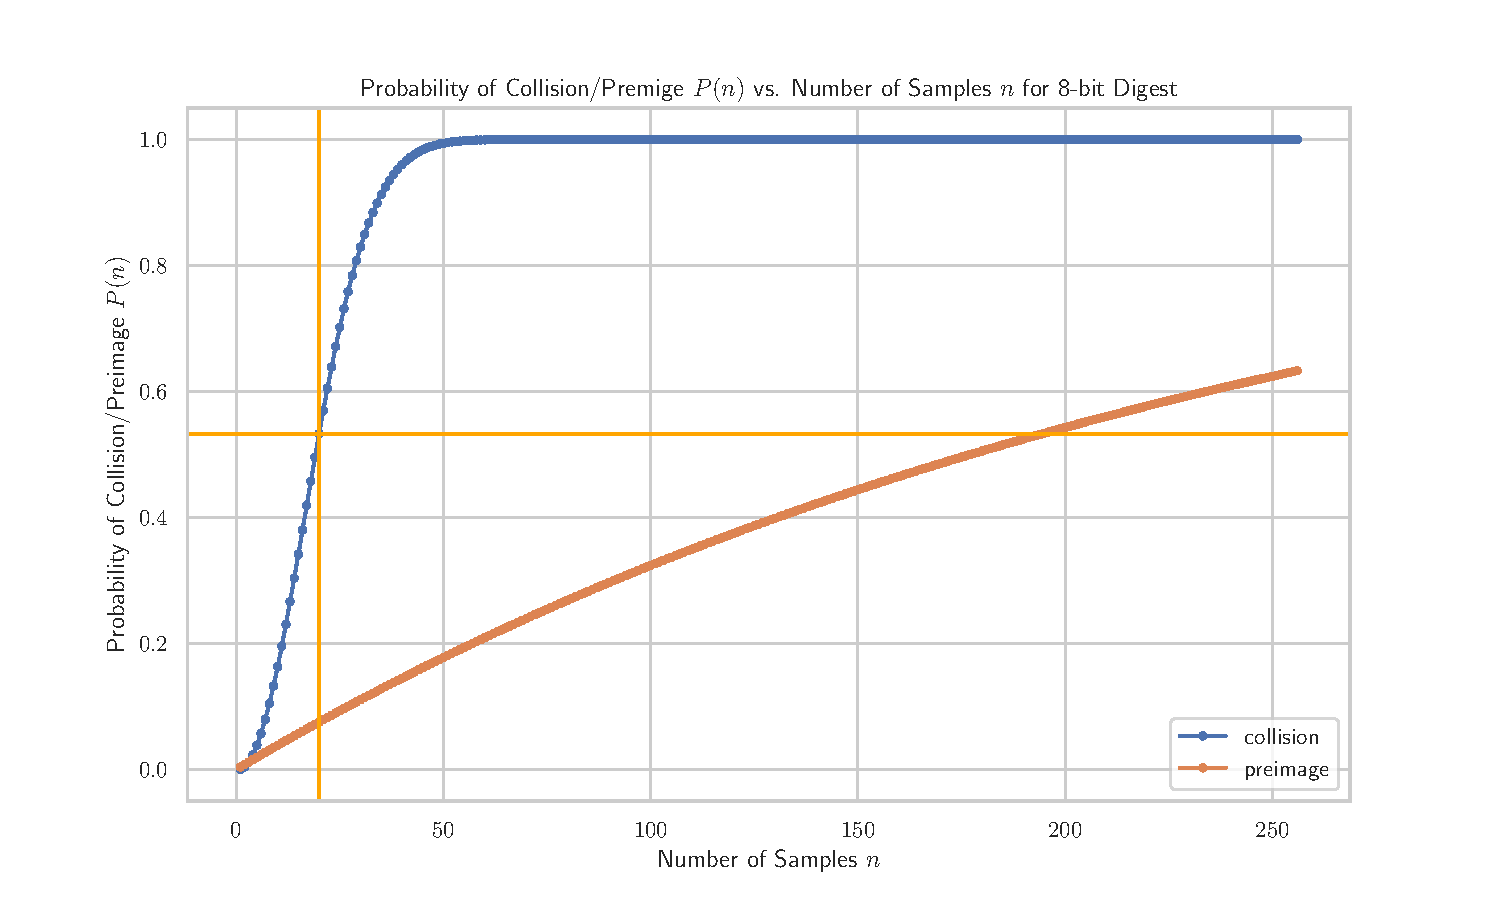
\includegraphics[width=\linewidth]{figure/birthday-paradox.pdf}
\captionsetup{width=.8\linewidth} 
\caption[Birthday Paradox with 8 Bits]{For a sequence of uniformly random draws of 8 bit numbers probability of at least one collision/preimage after $n$ draws $P(n)$ is compared to $n$. The orange cross-hair marks $P(20)$.}
\label{fig:birthday-paradox-8bits}
\end{figure}

It turns out that after only about $3.3\times10^{14}$ 96 bit \nonce s the probability of a collision reaches 50\%. While this is still a large number, if a protocol used a widely shared secret key $k$, and there were many (say billions) of clients using the same key, the chances of a \nonce reuse become high.
% Reusing a \nonce breaks confidentiality for \ac{AEAD} ciphers, and has even worse consequences for \ac{AES}-\ac{GCM}.

% [ ] \cite{aesgcm-security} attacker's advantage

\subsubsection{Nonce Brittleness}
\label{sec:nonce-brittleness}

Reuse of a $(\nonce,k)$ pair with AES-GCM destroys the confidentiality of the messages protected by that $(\nonce, k)$ pair. But for AES-GCM the consequence of $(\nonce,k)$ reuse is even worse, it allows an attacker to compute an underlying value $H$, which is used in all operations with key $k$ (even with a different \nonce). Possession of $H$ allows an attacker to forge messages, i.e. create cipher texts with valid authentication tags \cite[Section 5]{aesgcm-security}.

% [x] AES-GCM GHASH brittleness: using a (nonce,key) more than once allows an attacker to recover $H$ which means the attacker can forge messages forever (but does this mean the attacker can only forge when plaintext is empty?)

\section{HKDF}

The \acp{HKDF} described in RFC 5869 \citep{rfc5869hkdf} are used ubiquitously in the \ac{TLS} 1.3 protocol for the derivation of various traffic encpytion keys from the \ac{DHE} secret.
Additionally \ac{HKDF} is proposed to be used for the \ac{ECH} \var{accept\_confirmation} 8 byte acceptance signal (see e.g. Section 7.2 of \cite{esni}).

The \ac{HMAC}, standardised in RFC 2104  \citep{rfc2104}, is a pattern for performing message authentication based on cryptographic hash functions, and the authentication is secured with a secret key. The pattern works with any iterative cryptographic hash function. % TODO: what's an iterative cryptographic hash
A \ac{HMAC} scheme enables the calculation of the \ac{HMAC} digest over data with a secret a key, and verification that the \ac{HMAC} matches the data and secret key.
A successful verificatoin of the \ac{HMAC} digest
implies that the data have not been tampered with (with high probability),
and that the \ac{HMAC} was calculated by someone who knows the secret key (with high probability).

The \ac{HKDF} scheme is all about using a \ac{HMAC} to transform some \ac{IKM} (some source of secret randomness/entropy)
into a set of (yes multiple!) pseudo-random cryptographic keys.

Key derivation is carried out in two stages: \var{HKDF-extract} and \var{HKDF-expand}.
If the \ac{IKM} is already cryptographically strong and of the appropriate length, e.g. if the \ac{IKM} is a random string of \var{Hash.length} bytes,
then the \var{HKDF-extract} stage can be safely skipped and the \ac{IKM}
can be transformed
directly into a sequence of pseudorandom keys using successive applications of the \var{HKDF-expand} function.
It is possible, however, that the input keying material may be too long to be directly used in the \var{HKDF-expand} function, or it may not be cryptographically suitable, e.g. the \ac{DH} value $g^{xy}$ is not uniformly random and therefore not suitable as a PRK for the HKDF-Expand step.
So long as the \ac{IKM} contains sufficient entropy (read randomness), we can extract an appropriately long, uniformly (pseudo)random key from the \ac{IKM} by applying the HKDF-extract function.
For simplicity, when protocols use the extract-then-expand pattern, one can decide to always apply the HKDF-Extract stage, even if it is not always cryptographically necessary.

The \var{HKDF-Extract} function (the first step in the HKDF pattern) takes as input a salt (a non-secret random value) and the \ac{IKM} to produce a \ac{PRK}.
The salt is optional and is set to all zeros if not provided to the function, but is highly recommended in RFC 5869 Section 3.1.
Ideally the salt should be a random string,
and must have length equal to the length of the output of the underlying hash function used.
The second step is the \var{HKDF-Expand} function
which takes as input a \ac{PRK},
an optional information string (termed the label in \ac{TLS} 1.3),
and the desired length of the output,
to produce the \ac{OKM}.
The \var{HKDF-Extract} function is implemented as
\verb|HKDF-Extract(salt, IKM) = HMAC-Hash(salt, IKM)|, where the salt is being used as the `key' for the \var{HMAC-Hash} (but it does not have to be secret)
and the \ac{IKM} is the `input message' of the \var{HMAC-Hash} function.
This means that the \ac{IKM} can have arbitrary length. The \ac{OKM} is generated recursively as \[T(n) = \text{\var{HMAC-Hash}}(\text{\var{PRK}}, \text{\var{concatenate}}(T(n-1), \text{\var{info}}, n))\], \[\text{\var{OKM}}=\text{\var{concatenate}}(T(1),T(2),\ldots)\]
but where $T(0)$ is an empty string.
This recursive pattern means that the \ac{OKM} can be very long.
The info parameter in \var{HKDF-Expand} can be used to bind the \ac{OKM} to particular contexts, e.g. in \ac{TLS} 1.3 the client-to-server and server-to-client encryption keys are generated with different info parameters, i.e. each key is unidirectional. 

\section{HPKE}
The basic mechanism of \ac{ECH} is to encrypt the \ac{ECHI} with a randomly generated secret symmetric key, and then encrypt the symmetric key using the public key of the ECH server.

This pattern of encryption-to-a-public-key has been standardised by the \ac{IETF} as \ac{HPKE} in RFC 9180 \citep{rfc9180hpke},
and \ac{ECH} uses \ac{HPKE} ciphersuites exclusively
for \ac{CH} encryption.

A \ac{HPKE} suite consists of three components, the \ac{KEM}, the \ac{AEAD}, and the \ac{HKDF}.

\section{ The Diffie-Hellman Key Exchange }
The \ac{DH} key exchange protocol allows two parties, Alice and Bob, to establish a secret shared key
while communicating over an insecure channel \cite{diffie-hellman-1976}.
Variants and evolutions of the \ac{DH} key exchange protocol, in partical (\ac{EC})\ac{DHE},
are fundamental to how \ac{TLS} works.

An \ac{DH} key exchange involves Alice sending a \var{key\_share} to Bob, and Bob sending a \var{key\_share} to Alice. Both parties combine the two \var{key\_share}s in order to derive a shared secret which an eavesdropper cannot derive.

The original \ac{DH} key exchange was based on the
`apparent difficulty of computing logarithms over a finite field $GF(q)$ with a prime number $q$ of elements' \cite[p. 8]{diffie-hellman-1976}.
A finite field (a.k.a. Galois field), has a finite number of elements on which addition and multiplication are defined such that an additive inverse exists for all
elements and a multiplicative inverse exists for every nonzero element.
The integers with modular arithmetic modulo a prime number give us a finite field.

The \ac{DH} key exchange on finite field $GF(q)$ works as follows.
Alice and Bob each generate a secret independent random number $X_a$ and $X_b$ chosen uniformly from ${1,2,\dots,q-1}$.
Alice and Bob agree on a public value $g$, and each compute another public value $Y_i=g^{X_i}\mod q$.
Alice acquires $Y_b$ from Bob over an insecure channel, and vice versa.
% The original \ac{DH} description does not specify how Bob authenticates ownership of $Y_b$.
Alice and Bobs' shared secret is defined as $K_{ab}=g^{X_aX_b}\mod q$.
Alice computes this as $Y_b^{X_a}\mod q$ which is equivalent to Bob's $Y_a^{X_b}\mod q$.
Thus, Alice and Bob now each posses the shared secret $K_{ab}$.

When attacking \ac{DH} passively we observe $g$, $q$, $Y_a$, and $Y_b$.
We know that $Y_a=g^{X_a}\mod q$, and therefore that
\begin{equation}
\label{discrete-log-problem}
X_a=\log_g Y_a \mod q
\end{equation}
but it is computationally expensive to solve for $X_a$.
Equation~\ref{discrete-log-problem} is known as the discrete-log problem.
If a practical algorithm were discovered to solve the discrete-log problem efficiently,
i.e. with less than exponential complexity, then the \ac{DH} key exchange would be rendered ineffective.

Algorithms for solving the discrete-log problem do of course exist, so in order to use \ac{DH} securely in practice we have to choose a large enough $q$ such that computing the discrete-log becomes excessively expensive.
Unfortunately, choosing a large $q$ also entails a higher computational overhead for the benevolent parties, Alice and Bob.
Because of the mathematical relationship between the public and private values in \ac{PKC} it is generally the case that larger keys are required for \ac{PKC} than for symmetric cryptography in order to achieve the same security.

\subsection{DHE}
A problem with static \ac{DH} is that it is not forward secret. This means
that if one of the private keys is compromised then all past communications
based on the two \ac{DH} key pairs are compromised.
To combat this \ac{DHE} is a variant of \ac{DH} in which both public/private key pairs
are generated fresh for each connection. This means the security of each connection is more independent of the security of all past and future connections, i.e. compromising
the key of one connection does not necessarily compromise any other connection.
The \ac{TLS} 1.3 only allows ephemeral key exchanges. The only case in which \ac{TLS} 1.3 does not provide forward secrecy is when using an external \ac{PSK}.

\subsection{ECDHE}
\ac{EC}\ac{DHE} is a family of key exchange methods based on the mathematics of \ac{EC}
rather than finite fields.
For example, the Curve25519 crypto system is based on the elliptic curve $E$ defined by
$y^2=x^3+486662x^2+x$ and uses the Galois field $\mathbf{F}_p$ with prime number $p=2^{255}-19$.
Elliptic curve cryptography is based on a special definition for the addition
of two points on an elliptic curve $E$.
Say $P$ is on the curve $E$; $P\in E$,
then our special addition operation entails that $P+\ldots+P=kP\in E$. 
The difficulty of breaking elliptic curve cryptography is then based on
the computational complexity of finding $k$ given $Q=kP$ and $P$,
i.e. solving the elliptic curve discrete log problem.

\ac{X25519} is a \ac{EC}\ac{DHE} sytem based on Curve25519,
and it has several desirable properties,
including the fact that for \ac{X25519} as a \ac{KEM} the \var{enc} value
is a 32 byte value,
where all possible 32 byte values are valid public keys.
While it may be possible to distinguish between a long stream of \var{enc} values compared to a long stream of uniformly random 32 byte values,
the number of values needed to make this distinction would be large.
One of our designs for \ac{SECH} will make the assumption that
distinguishing between an \ac{X25519} \var{enc} and a truly random
value is hard enough such that detection is computationally infeasible

\section{TLS 1.3}
A \ac{TLS} 1.3 connection is initiated by the client's \ac{CH} message, which (usually)
contains an (\ac{EC})\ac{DHE} \var{key\_share}.
The server responds with its \var{key\_share} in the \ac{SH} followed by the first flight of encrypted messages: \ac{tlsEE}, \ac{tlsC}, \ac{CV}, and \ac{tlsF}.
After constructing the \ac{SH} the server can compute the server handshake traffic secret using \ac{HKDF}. The authentication messages \ac{tlsEE}, \ac{tlsC}, \ac{CV}, \ac{tlsF}, are all encrypted under \ac{AEAD} using this secret.

Upon receipt of the \ac{SH} the client also has enough information to construct the server handshake secret, and thus to decrypt the incoming authentication messages.
The client finally constructs the \ac{tlsF} message which contains a \ac{MAC} digesting the entire transcript of messages up to that point.

Since both parties verify each others \ac{tlsF} message, they are assured that the agreed keys and parameters have not been tampered with by a \ac{MITM}.

The flow described above is just one of various possible flows.
This flow involves just one full round-trip (one flight of messages from the client, one from the server) before the client can start sending application data.
The server can start sending messages after the third flight has been processed.

\subsection{Early Data}
\ac{TLS} 1.3 also permits application in the first flight of client messages (called 0\ac{RTT} data),
but the protection of the `early data' is weaker,
in particular 0\ac{RTT} data is not protected against replays.
If the server processes the `early data' and passes it to the application
before the handshake has completed, then the application
may be processing maliciously replayed data (see Appendix~E of \cite{esni}).

\subsection{The \var{HelloRetryRequest} Message Type}
With TLS 1.3 the server can (hopefully in an overwhelming majority of cases) generate the application traffic key after processing just one flight of messages from the client. This is possible because the client `guesses' an (\ac{EC})\ac{DHE} curve/group and sends an appropriate \var{key\_share} in the \ac{CH} (in fact the client may send multiple \var{key\_share}s for multiple curves/groups to increase the probability that the server will support at least one of those cipher suites).
However, if the client guesses wrong and sends a \var{key\_share} for a curve/group not supported by the server,
then the server should respond with a message that informs the client as to which curves/groups are supported.
This subsequent message is called the \ac{HRR}.

The \ac{HRR} message format is designed to look almost identical to the \ac{SH} message for compatibility with hardened \ac{TLS} 1.2 middleboxes that fail to correctly ignore new message types for the first server message.
From the perspective of a middlebox
that is unaware of \ac{TLS} 1.3
the \ac{HRR} is treated just like a \ac{SH},
but the client can distinguish between \ac{HRR} and \ac{SH} based on a special value in the \var{random} field of the message
(which we would call the \var{ServerHello.random} if we interpreted the \ac{HRR} as a \ac{SH}).

\begin{listing}
    \centering
    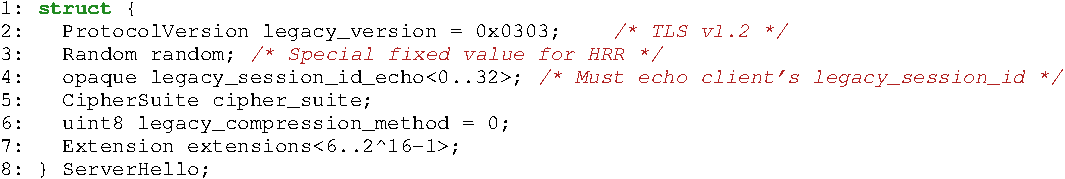
\includegraphics[width=\linewidth]{figure/ServerHello-struct.pdf}
    \captionsetup{width=.8\linewidth} 
    \caption[\ac{SH} and \ac{HRR} Structures]{The structure of the \ac{SH} message, which is the same as the structure of \ac{HRR}, repeated from Section 4.1.3 of \cite{esni} using the presentation syntax defined by same.}
    \label{lst:server-hello-struct}
\end{listing}

The use of the special constant value in the \var{random} field of the \ac{HRR} has implications for the design of the \ac{ECH} protocol.
In the happy case when the server accepts the first \ac{CH}
(it supports the curves/groups for the \var{key\_share} etc.),
and when the server also accepts \ac{ECH}, then the last 8 octets of the \ac{SH}\var{.random} are filled with a special ECH acceptance signal.
But, in the case where \ac{HRR} is necessary and \ac{ECH} is accepted
the last 8 octets of the \ac{HRR}\var{.random}
are not available because they are used to distinguish that the message is a \ac{HRR} and not a \ac{SH}.
Instead, in the case of \ac{HRR} {\em and} \ac{ECH} acceptance
the \ac{ECH} 8 byte acceptance signal is put in the
\var{ECHClientHello.payload} field of an \var{encrypted\_client\_hello} extension
(as described in Section 7.2.1 of \cite{esni}).
Using a distinct extension to deliver a stealthy acceptance signal
would not be acceptable because it would stick out.

\subsubsection{Can we put a stealthy signal in the \var{HRR}?}

Let's consider a \ac{TLS} session in which a \ac{HRR} is triggered.
An easy way to achieve this practically is to set up a TLS 1.3 server which only supports an uncommon (\ac{EC})\ac{DHE} group such as P-384.
Most clients (including \var{openssl s\_client}) will not provide a P-384 \var{key\_share} by default in the ClientHello,
and the server will respond with a \ac{HRR} with a \var{key\_share} extension selecting \var{KeyShare.selected\_group = secp384r1}.
Note that the server-to-client \var{key\_share}
in a \ac{HRR} message contains only an indication of the type of key share the server supports,
but does not include a \var{KeyShareEntry}.
The total number of bytes in the \var{key\_share} extension in a HRR message is 6, 2 for the extension length, 2 for the extension type, and 2 for the \var{SelectedGroup} field. Therefore, there is no room in the HRR server-to-client \var{key\_share} to embed a stealthy ECH/SECH acceptance signal. The other extension that will be present in the \ac{HRR} is the \var{supported\_versions}, which also has a length of 6 bytes, none of which can be manipulated stealthily.

Another option for sneaking an acceptance signal in the \ac{HRR}
could be to use the \var{cookie} extension as cover.
The cookie extension (identified by \var{0x002C})
allows the server to send arbitrary data
(of length $1$ to $2^{16}-1$ bytes) in either the \ac{HRR} or the \ac{SH}.
In accordance with \cite{rfc8446} when a client processes a cookie in an \ac{HRR}
it must echo the cookie extension exactly in the subsequent \ac{CH2} message.

Since the cookie extension is allowed in \var{HRR} messages and can contain opaque data it can be used to send a secret acceptance signal.
However, the cookie extension is not mandatory and may be used differently
(or not used at all) by different servers.
Thus, in order to successfully achieve a {\em stealthy} acceptance signal via the cookie, the extension would have to be manipulated in such a way that it does not stick out  when compared to normal \ac{TLS} traffic,
or \ac{TLS} traffic in the environment would have to be \ac{GREASE}'d.
For instance, the length of the cookie must not be an indicator of whether the cookie contains an acceptance signal.
Also, if the cookie were to be used for the acceptance signal a censor could block all connections that use \ac{HRR} cookies in order to thwart \ac{SECH}.

\cite{rfc8446} mention two purposes for the cookie extension;
\begin{enumerate}
    \item \ac{DoS} Mitigation: Forcing the client to echo back the cookie allows the server to verify that the client is `live', which increases the cost of (and thus mitigates) \ac{DoS} attacks.
    \item Offloading State: The cookie extension allows the server to `offload state' to the client, i.e. to ask the client to manage some data pertaining to the \ac{TLS} connection. By offloading state to the client the server can determine which messages belong to the same connection while running statelessly.
\end{enumerate}
If the \ac{HRR} cookie is used to hide an \ac{SECH} acceptance signal it interferes with these two capabilities.


% TODO repetition
For a design of a stealthy \ac{ECH} protocol we require that the \ac{SECH} acceptance signal also be stealthy.
For \ac{ECH} the acceptance signal is stealthy in the case that \ac{HRR} is skipped, but it is not stealthy when \ac{HRR} occurs.
To facilitate \ac{HRR} while performing \ac{SECH}
we would need a new mechanism to sneak the \ac{SECH} acceptance signal to the client.
One approach would be to delay the SECH acceptance signal until the true \ac{SH},
and put the \ac{SECH} acceptance signal
in the \var{ServerHello.random} field.
Another approach would be to use any other available random bytes in a typical \ac{HRR} and replace them with the acceptance signal.
As discussed there are no high-quality random bytes available
in the \ac{HRR}.
The \ac{HRR} cookie is not universally
present and can be used differently by different servers,
so leveraging the cookie without sticking out is difficult.

As we'll discuss in Section~\ref{sec:hrr-hijacking}
it turns out that facilitating the \ac{HRR} flow
for \ac{SECH} while maintaining stealth
is rather tricky due to \ac{HRR} hijacking.
For this reason in this work we have decided to drop the
goal of facilitating \ac{HRR} for \ac{SECH},
which means we only have to worry about
the \ac{SECH} acceptance signal
for the \ac{SH} message.

\subsection{Tickets and Session Resumption}

A TLS 1.3 server can issue tickets to clients after successful completion of a handshake.
These tickets allow a client to initiate new \ac{TLS} 1.3
sessions with the client and achieve server authentication
with fewer messages (no \ac{tlsC} nor \ac{CV}).

% TODO repetition
The motivation for the \ac{TLS} 1.3 ticket system
comes from the typical behaviour of web browsers when loading and rendering web pages.
Many contemporary web pages rely on a large number of resources to be loaded from the server.
With the \ac{TLS} ticket system it is typical for a \ac{HTTPS} server
to issue several tickets (e.g. 6 or more) for every successful handshake.
This means that when a web browser is loading a web page it can first complete a full handshake,
and then open several more TLS connections to the server concurrently
in order to load subsequent resources more quickly (e.g. images, videos, JavaScript files).

% [ ] Details of tickets as specified by TLS 1.3 RFC. \var{psk\_binder}, \var{NewSessionTicket} message type, what happens when multiple servers have authority on the server's certificate?

% [ ] the \var{pre\_shared\_key} extension
The structure of the \var{pre\_shared\_key} extension as defined in Section 4.2.11 of \cite{esni} is repeated in Listing \ref{lst:psk-struct}.
When the client offers \var{pre\_shared\_key} it contains a list of (\var{identity}, \var{binder}) pairs,
and if the server accepts \ac{PSK}-based key establishment it sends back just the index of the selected identity.
The \var{pre\_shared\_key} extension is exceptional in that it
"MUST be the last extension in the \ac{CH}" (\citet[Section 4.2]{esni}).
This restriction makes implementation of the \var{binders} slightly easier because each binder in \var{binders} is a \ac{HMAC} incorporating the entire \ac{CH} up to but excluding the list of \var{binders} themselves.

% The \var{PskIdentity} structure has an opaque \var{identity} field of between $1$ and $2^{16}-1$ bytes, which is plenty of room for stealthily sending encrypted data.

\begin{listing}
    \centering
    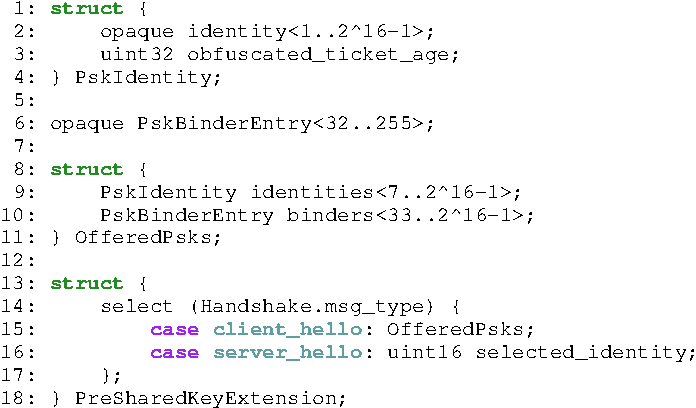
\includegraphics[width=.8\linewidth]{figure/pre_shared_key.pdf}
    \captionsetup{width=.8\linewidth} 
    \caption[Structures for the \var{pre\_shared\_key} extension]{TLS 1.3 presentation language representations of the structures used for the \var{pre\_shared\_key} extension.}
    \label{lst:psk-struct}
\end{listing}

The \ac{PSK} system has the potential for use as stealthy cover,
but in this work we pursue a design that instead uses \ac{PSK}s as way
of bootstrapping or distributing access to an \ac{SECH} server.

% [ ] Stateful/stateless cookies.

% [ ] Notes about how tickets are typically used in reality. Notes about any strict restrictions on the ticket behaviour in TLS 1.3 RFC.

% [ ] Introduce idea of using tickets to distribute access to an SECH server (will this be a way to distribute a symmetric key, or can the ticket allow a one-time connection that does not require the symmetric key?).

\subsection{ECH}

\subsubsection{\var{ECHConfig}}
The \var{ECHConfig} is a public value containing a public key and other parameters
which an \ac{ECH} client needs in order to offer \ac{ECH}.

% ECHConfig structure and fields
\cite{esni} define (in Section 4) just one version (identified by the hextet \var{0xFE0D}) of the \var{ECHConfig}, but  the structure is defined in a way that will compatibly allow future versions.
The interesting part of the \var{ECHConfig} is the \var{ECHConfigContents} which has four fields,
the \var{key\_config}, the \var{maximum\_name\_length}, the \var{public\_name}, and \var{extensions}.
The \var{key\_config} contains the \var{public\_key} needed by a client to encrypt the \ac{CHI} under \ac{HPKE}.
As well as the \var{public\_key} the \var{key\_config} has a \var{config\_id},
a \ac{KEM} id (\var{kem\_id}) and a list of \ac{HPKE} symmetric cipher suites supported by the \var{ECHConfig}.
The \var{config\_id} is ``A one-byte identifier for the given \ac{HPKE} [public] key''.

% hard to send config\_id stealthily
When a client offers \ac{ECH} it sends the \var{config\_id} of the public key used to encrypt the ClientHelloInner.
This \var{config\_id} means that the server only has to attempt decryption of the \ac{CHI} once,
which is essential for a scalable deployment of \ac{ECH},
supporting convenient regular config rotation.
In the case of a stealthy \ac{ECH} variant, however, transmitting a \var{config\_id} stealthily in the first flight of messages from the client (without permitting an attacker to detect the \ac{SECH} \var{config\_id}) is a challenge.
For this reason we will likely have to accept a less scalable approach
to \ac{SECH} key management and rotation.

For \ac{TLS} the client just needs the servername and IP address to access the server,
but for \ac{ECH} the client additionally needs the public key of the \ac{ECH} backend server.
The \var{ECHConfig} will typically be distributed using \ac{DNS} alongside the server \ac{IP} address,
which means that the \ac{ECH} backend server will be advertising its own existence to users and censors alike.
But other ways of distributing \ac{ECH} configurations
such as having the \var{ECHconfig} preconfigured in the client, are also permissable.

Since the \ac{ECH} protocol is not stealthy there is little harm done in advertising the existence of the \ac{ECH} backend server,
it would be possible for a powerful attacker to enumerate \ac{ECH} backend servers with high confidence using \ac{DPI}, traffic analysis, and active probing.

For \ac{SECH} we have an opportunity to hide
the existence of backend \ac{SECH} servers from attackers,
which may be particularly beneficial for censorship-circumvention use cases.
If the existence of the backend \ac{SECH} server can be hidden from potential censors then the anonymity set for \ac{SECH} connections becomes the entire set
of all \ac{TLS} 1.3 servers on the Internet,
creating a very strong incentive against overblocking in order to block \ac{SECH}.




% CLIENT                            CF-SERVER                             BACKEND SERVER
% ClientHelloOuter
% +encrypted\_client\_hello
% --------------------------------------->
%                                          ClientHelloInner
%                                          ------------------------------->
%                                                               ServerHello
%                                                      +accept\_confirmation
%                                          <-------------------------------
%                              ServerHello
%                     +accept\_confirmation
% <---------------------------------------

\subsubsection{ECH acceptance}

As noted above the \ac{ECH} acceptance signal is embedded into the first message sent by the server,
whether the first message is a \ac{SH} or a \ac{HRR},
however the location of the message is different in the \ac{HRR}.
This difference is an unfortunate added complexity.
An alternative design might have had the \ac{ECH} acceptance signal always embedded in the \ac{SH}, whether or not a \ac{HRR} is issued.
One reason such a design is not acceptable for \ac{ECH}
is that the client needs to know whether a message it is processing was constructed by the client-facing server or the backend server,
including whether the \ac{HRR} was sent by the client-facing or backend server.
To prevent certain kinds of attacks and to minimize bandwidth,
\ac{ECH} is designed so that
the client can abort the connection as soon as possible
if \ac{ECH} is rejected. % TODO: this is not quite right

% If the \ac{HRR} is constructed by the client-facing server (i.e. ECH was rejected),
% then the \ac{HRR} corresponds to the ClientHelloOuter,
% but if the \ac{HRR} was constructed by the backend server then it corresponds to the \ac{CHI}.
% In order for the client to construct a valid \ac{CH2} it needs to know which ClientHello message the HRR is rejecting.
% While it may have been possible for a client to infer from the HRR contents (without an ECH acceptance signal) which ClientHello message it corresponds to (e.g. by process of elimination on the supplied cipher suites in either CH), this approach would not be robust and would make extensions to the protocol more complicated yet. Also, without the ECH acceptance signal it may be more difficult to analyse the security properties of the protocol due to an increased number of possible states the client can be in after processing the HRR.
% Also, according to \cite{esni} when a client offers ECH but the server does not accept then the client must terminate the connection with a \var{ech\_required} alert, which is not encrypted and thus transparent to network observers. In order to reduce the amount of unnecessary traffic ECH is designed so that the client can decide whether to emit the terminal \var{ech\_required} alert upon receipt of first server message.
A stealthy variant of \ac{ECH} should not conspicuously terminate the connection when \ac{SECH} is rejected,
but ought to either continue with the handshake or emit an inconspicuous alert in order to conceal the fact that \ac{SECH} was attempted.

It turns out that to maintain stealth the \ac{SECH} acceptance signal
needs to be cryptographically stronger than the
relatively weak 8 byte \ac{ECH} signal.
In particular, a preimage of the \ac{SECH} acceptance signal
could be used to trigger a client reaction that reveals \ac{SECH} is being attempted.
We propose a 24 byte \ac{SECH} acceptance signal embedded in the \ac{SH}\var{.random}.
This means the signal can have better pre-image resistance
than the 16 byte \ac{AES}-\ac{GCM} verification tag, 
which is in widespread use in \ac{TLS}.
The reason to use only 24 bytes rather than all 32 is to leave room for the possibility of running both \ac{SECH} and \ac{ECH} over the same connection.

\includefigure{fig:ech-reject-and-hrr}{
    Sequence Diagram of \ac{ECH} Rejection and \ac{HRR}}
    {
    A sequence diagram for a session in which the client attempts \ac{ECH} but \ac{ECH} is rejected {\em and} the parameters of the \ac{CHO} aren't supported (hence \ac{HRR}).
    Since \ac{ECH} is rejected the client responds with a fatal \var{ech\_required} alert in compliance with Section~5 of \cite{esni}.}{figure/ech-reject-and-hrr.pdf}

\section{Considering a stealthy variant of ECH}
\subsection{Finding cover in TLS 1.3}
\label{sec:sech-cover-constraints}
We can potentially use any parts of the TLS 1.3 \ac{CH} message that look (or are) random,
as stealthy cover.
However, the quality of the cover depends on the
various factors,
such as whether the field is necessary (i.e. always present in clients first flight of messages),
whether the size or structure of the field
is implementation dependent,
and whether the semantics of the field can be used
to mount an attack that destroys stealth.

For our purposes we are looking for cover that does not depend
on the use of \ac{GREASE}. Our conclusion is that the \var{random}
and \var{legacy\_session\_id} are the only parts of the client's first flight
of messages providing good stealthy cover that does not need to be \ac{GREASE}'d.

\subsubsection{The \var{random}}
The \ac{CH}\var{.random} contains 32 random bytes, the purpose of which is to
ensure freshness of both the handshake and application symmetric keys
and the server's \ac{CV} message,
in order to prevent replay attacks.
The \ac{CH}\var{.random} provides high quality cover,
but using non-random values in its place could impact the security of the handshake.
We posit that it may be cryptographically sound
to replace the \ac{CH}\var{.random} with ciphertext
since the ciphertext will be just as unpredictable as a random value from the perspective of an attacker.
However, it is beyond the scope of this project to
provide a formal or mechanistic attestation of this.
In \ac{TLS} 1.3 the \ac{CH2}\var{.random} must match the \ac{CH}\var{.random} if it exists.

\subsubsection{The \var{legacy\_session\_id}}
The \ac{CH}\var{.legacy\_session\_id} also consists of 32 random bytes.
Its purpose
is to maintain compatibility with misbehaving
middleboxes,
it is essentially an example of the \ac{GREASE}
technique.
This field offers the highest quality cover because it is always present and plays no particular
role in the cryptographic negotiation.
The \var{legacy\_session\_id} is in fact intended to make \ac{TLS} 1.3 `look like' an earlier version of \ac{TLS},
and in our design we will use it to make \ac{SECH} `look like' \ac{TLS} 1.3.

\subsubsection{PSK}
Clients may send an arbitrary number of \acp{PSK}
identities in their \ac{CH}.
These identities can, for example, be self-encrypted ciphertexts created by the server
in a previous session.
Alongside each \ac{PSK} there must be a \var{binder},
which is a \ac{MAC} binding the use of the \ac{PSK} to the current session as well
as the session in which the \ac{PSK} was created.
Both the  \var{identities} field and \var{binders} field
have potential to be used as cover for \ac{SECH},
with the one caveat that the \ac{PSK} extension is not always present
in a \ac{CH}.
Relying on the \ac{PSK} for cover thus reveals a small amount of information
to an attacker about whether or not \ac{SECH} is being run.
Also, the size of the \ac{PSK} extension fields will vary between different
implementations and configurations,
meaning some empirical research would be needed in each deployment
in order to use the \ac{PSK} as cover in a way that does not stick relative
to the environment.

For these reasons we are pursuing in this work a design that does not use
the \ac{PSK} field as cover,
but we note that it remains a good option to pursue in future research,
in particular in order to expand the bandwidth of the \ac{SECH} payload.
\subsubsection{The Client's \var{key\_share}}
The \ac{CH}\var{.extensions.key\_share} has a field called \var{client\_shares} which is defined to contain between $0$ and $2^{16-1}$ bytes of data,
which can be parsed into a list of 0 or more key exchange public parameters.
The structure of this field depends on the set of
(\ac{EC})\ac{DHE} curves/groups listed in the \var{supported\_groups} extension.
The \var{supported\_groups} are listed in descending order of preference,
and the \var{client\_shares} must be listed in the same order.
To take a concrete example, let's say that
the first value in the \var{client\_shares} list
is an \ac{X25519} key share of length 32 bytes,
and the second is a \ac{p256} key share of 65 bytes.
The 32 bytes of the \ac{X25519} are indistinguishable from random and thus provide good cover.
On the other hand the \ac{p256} has structure and would require
some finagling to be able to use it as cover stealthily.
Some values for the 65 bytes are not valid \ac{p256} key shares,
which an attacker could detect, so if a ciphertext took on one of those
impossible values, then an attacker could detect it.

If we use the \ac{X25519} key share as cover for ciphertext
then the key share value cannot be used for an actual key agreement,
since there is no associated private key with the fake public key (which is
actually ciphertext).
The problem with using the \ac{X25519} key share as cover is twofold:
1. it means we could not actually use the \ac{X25519} key exchange, and 2. it would expose us to an active attack that would destroy stealth.
That attack would work as follows. A client replaces the key share
value with ciphertext. The \ac{CH} is intercepted by an active attacker
who attempts to complete the key exchange using the client's fake key share.
The client does not have a private key and cannot compute the shared secret value
meaning the client cannot derive the handshake traffic secrets,
and in turn cannot decrypt the \ac{tlsEE} or \ac{tlsC} messages.
The attacker can leverage this to use the client's reaction as an oracle
to reveal that \ac{SECH} was attempted.
%The point at which the client should abort the handshake is when the attacker
%sends an invalid \ac{CV},
%since the attacker does not possess
%the private key associated with the \ac{tlsC}.
For example, if the attacker purposely sends a corrupted record the client should respond
with a \var{bad\_record\_mac} alert.
But with a properly formatted,
though invalid, \ac{CV} message the client
should respond with a \var{decrypt\_error} alert.
Without the handshake traffic secret the client is unable to determine
which response is appropriate,
so the client's reaction reveals that
the \ac{X25519} key share was fake.

For this reason we determine that the \var{key\_share} extension does
not provide cover for \ac{SECH} under an active-attacker threat model.

\subsubsection{Early Data}
The early data mechanism has the potential to provide a lot of
cover for \ac{SECH} payloads.
The lack of protection against replay for early data is worrying,
but replay protection could be handled in the \ac{SECH} design.
Similar to \acp{PSK}, though, the use of early data is situation and
implementation dependent,
so avoiding sticking out would require empirical analysis of the environment
and/or \ac{GREASE}ing.
We do not pursue the use of early data as cover in our designs,
but similar to \ac{PSK} this approach has good potential
for a design where the tradeoff is to maximise bandwidth rather than stealth.

\subsubsection{The Padding Extension}
The padding extensions \var{extension\_data} field `consists of an arbitrary number of zero bytes'.
This padding could be used as cover for SECH by using the length of the \var{extension\_data} as a piece
of data itself. Say we use padding as cover for some bits and set the maximum padding size to 15, then
the size of the padding encodes 4 bits of data:
\begin{verbatim}
0  -> 0000
1  -> 0001
2  -> 0010
3  -> 0011
...
15 -> 1111
\end{verbatim}

The tradeoff between transmission size and stealthy bits is terrible here,
a padding extension of size 16 takes up 20 bytes (160 bits),
counting in the extension header, but offers only 4 covert bits.
Even worse, the total covert bits scales logarithmically with the maximum padding size.

The padding extension was introduced to solve issues with buggy implementations, and using
the padding extension for covert bits would require some engineering to ensure that the extension
could fulfill its original purpose.
Also, if the padding extension is used to encode covert bits (which may for instance be part of a cipher text),
then these covert bits will look uniformly random when tracked across sessions, which an attacker
could detect, thus compromising stealth.


\subsection{Offering Both ECH and SECH}
While it is not immediately obvious that offering {\em both} \ac{ECH} and a stealthy \ac{SECH} variant could be beneficial there are some circumstances where offering both may in the future be necessary to protect privacy or facilitate censorship circumvention.
In particular the risk that \ac{ECH} will be blocked outright by some powerful censors (e.g. in China),
means that the convenience and enhanced privacy of regular ECH may be preferable in regions where ECH is not blocked,
but the stealthy alternative may be the only way to access the domain privately from regions where \ac{ECH} is blocked.
This is a clear case where servers may in future wish to offer enable both \ac{ECH} and \ac{SECH}.

But offering these two methods for accessing a resource privately
is an inherent increase in complexity of the overall system compared to a system that only offers {\em either}
\ac{ECH} {\em or} \ac{SECH}.
This increase in complexity increases the attack surface of the system,
there will be more branches of code on both the client and the server,
the cost of developing and deploying the additional code will be significant,
and the simultaneous co-operability of the two protocols presents new challenges to the design of each.
That the two protocols should co-operate also introduces an additional burden of analysis in terms of identifying and mitigating attacks against each of the protocols.
For all of these reasons there is a strong temptation to pursue developing versions of \ac{ECH} and \ac{SECH} that are designed *not* to co-operate with each other.
However, another pattern of argument relevant to most security protocols emphasises the importance of having a stand-by backup option to a widely deployed algorithm.
For instance, the most popular/widely-deployed \ac{AEAD} algorithm on the internet is AES-128-GCM,
but many software packages also support ChaCha20-Poly1305 because it could transpire
at any moment that AES-128-GCM has a fundamental flaw and needs to be replaced urgently.
This argument can also be applied to \ac{ECH} and \ac{SECH};
it would be wise to have both options ready, well-analysed, and deployed such that either one can be quickly disabled in case a fatal security flaw is discovered.

The above argument pertains to the simultaneous
deployment of \ac{ECH} and \ac{SECH} for a single domain,
but what about having versions of \ac{SECH} and \ac{ECH}
that facilitate the server accepting both \ac{ECH} and \ac{SECH} within a single TLS session?
Is there a motivation for such a design?
Consider, for example, an enterprise network in which the enterprise has control of client devices and is able to manage the list of trusted \ac{CA}s on each client device.
In such a case the enterprise network administrator will be able to mount a \ac{MITM} attack,
which would allow inspection of the TLS 1.3 application traffic as well as the \ac{CHI} if \ac{ECH} is being used.
There is motivation for network administrators to enforce such a situation for various reasons,
e.g. the enterprise network may be attempting to thwart phishing campaigns, and the risks of phishing campaigns can be mitigated by blocking traffic to suspicious or known malevolent servernames.
We can foresee a scenario, then,
where the network administrator decides to mount a \ac{MITM} attack in order to inspect the encrypted \ac{CH},
but no other part of the \ac{TLS} 1.3 encrypted traffic.
Let's imagine now we have a client trying to circumvent this \ac{MITM} attack.
If \ac{ECH} is available and used by default then it would be suspicious for the client not to use \ac{ECH}. However, the client may observe that using \ac{ECH}
to connect to \var{blocked.example.com} gets blocked,
and therefore will have to access \var{blocked.example.com} by some other means.
In such a case the client would benefit from the ability to make a `cover' \ac{ECH} connection request (to \var{allowed.example.com}, say)
and simultaneously an \ac{SECH} connection request to \var{blocked.example.com}.
To accommodate this scenario we would like for it to be possible to attempt \ac{ECH} and \ac{SECH} on the same connection.

One of the side-quests for this dissertation was to design \ac{SECH} such that it could run under \ac{ECH}.
We have not ended up pursuing this goal,
but some design decisions were made with
this goal in mind.

%It seems unlikely, however, that there would be much benefit from the server being able to accept both ECH and SECH, since the acceptance signal for ECH is sent in the same flight as the server certificate. If ECH and SECH are both accepted by the server, but with differing inner servernames (e.g. `ech.example.com` and `sech.example.com`), the server will have to select a certificate to send for the same flight of messages as the ECH acceptance signal. Possibly, it would be beneficial to the client to know that both were accepted, such that it can decide how to try to establish subsequent connections. 

% \subsection{Accepting SECH}

% The \ac{ECH} acceptance signal is necessary
% because the client continues the handshake differently (e.g. the Finished message is constructed with a transcript using the ClientHelloInner) when it detects a positive ECH \var{accept\_confirmation} signal from the server. The design of the ECH acceptance signal facilitates ECH split-mode, in which the backend server only processes one ClientHello (ClientHelloInner if the client-facing server accepts ECH, and ClientHelloOuter otherwise).

% [ ] The purpose of an SECH acceptance signal is to inform the client as early as possible whether or not the server is intending to use the inner or outer servername. It is sufficient to include only a positive signal (the server is accepting the SECH inner servername), and to infer that the outer servername will be used when the positive signal is absent.
%     - Detecting the length of the domain name

% [ ] must not be possible for an attacker to detect the length of the inner servername, merely knowing the length of the servername could leak the servername itself

\section{Threat Models and Attacks}

The \ac{TLS} threat model assumes all messages
are mediated by an active attacker,
and for the most part the \ac{ECH} threat model is the same.
However, there are active attacks that distinguish
\ac{ECH} \ac{GREASE} from proper \ac{ECH}.
In this work we pursue designs of a stealthy \ac{ECH}
which cannot be distinguished from a normal \ac{TLS} 1.3 connection,
even in the presence
of an active on-path adversary.

Various potential attacks against \ac{ECH}
have been discovered.
In Section~\ref{sec:active-attacks} we discuss
each of the active attacks highlighted by \cite{esni}
and explain our approach to mitigating them in the case of \ac{SECH}.

\subsection{Bleichenbacher Attacks \label{bleichenbacher-attack}}
\cite{bleichenbacher1998chosen} demonstrated how an attacker could reveal the \premastersecret{} of an \ac{SSL} 3.0 connection when the \premastersecret{} is protected with \ac{RSA} public key encryption.
The effectiveness of the attack varied according to the specifics of the implementation, in particular the granularity of information revealed by the server about why a handshake is aborted.
The method, which is based on informatoin leaked by the server about decryption failure or incorrect formatting of plaintexts, was quite easily generalised and variants of the attack have been repeatedly found.
Also, \cite{boeck2018robot} showed that variants of the attack were still effective against a broad set of Internet servers, despite years of research and effort spent trying to plug leaks in protocols and implementations.
Therefore, in designing a new cryptographic protocol it would be remiss not to account for this type of attack.

\citeauthor{bleichenbacher1998chosen}'s (\citeyear{bleichenbacher1998chosen}) adaptive-chosen-ciphertext attack against \ac{RSA} when using  \ac{PKCS} \#1 standard concerns the situation where
the \ac{RSA} public key $n,e$ and the ciphertext $c$
are known to an attacker who wants to recover the secret message, $m=c^d\mod n$, or even
the \ac{RSA} secret key $d$.
In \ac{PKCS} \#1 the secret message is padded to the length of $n$, including a fixed prefix \var{0x00 0x02}.
By sending a malicious ciphertext $c'\equiv cs^e\mod n$, where $s$ is chosen adaptively, if a server reveals that the corresponding plaintext $m'=c'^d\mod n$ is correctly formatted, then the attacker knows the first two bytes of $m'$ are \var{0x00 0x02}.
By cleverly using this information in adapting successive choices of $s$ they find that for a 1024-bit modulus $n$ the expected number of oracle accesses needed to recover the secret message is about 1,000,000, which is reasonably low and hence enables practical attacks.

A primary goal of the \ac{SECH} protocol is to maintain confidentiality of the very fact that \ac{SECH} is being attempted\footnote{connection-level \ac{PC}},
and also confidentiality of whether the server supports \ac{SECH}\footnote{channel-level \ac{PC}}.
Care must be taken, therefore, to ensure that responses (or lack of a response)
from a server,
such as an alert about encryption or formatting errors,
as well as the timing of those responses,
do not reveal information about whether:
1. the server supports \ac{SECH} at all, and
2. the client attempted \ac{SECH} in the given connection.


\chapter{Design}
\label{chap:Design}

\section{Considerations for split-mode SECH}
[ ] reminder: what is split-mode?

\cite{esni} describe two modes of operation for ECH, shared mode and split mode. In shared mode there is a single server which performs the ECH decryption {\em and} terminates the TLS connection, whereas in split mode there is a client-facing server that performs ECH decryption and which proxies the remaining TLS traffic to and from a backend server which terminates the TLS connection. For ECH each server is `aware' of its role in the ongoing connection. The server can have a different role for different connections, but within the context of a single connection the server determines its role based on the \var{type} field of the received \var{encrypted\_client\_hello} extension, if the \var{type} is outer then the server is the client-facing server, if it is \var{inner} the server is the backend server.

[ ] motivations for split-mode: 1. distribute workload, 2. enhanced privacy for backend server (client-facing server can't see application traffic)

[ ] reasons for hesitance in deploying split-mode: 1. low incentive for large providers (the provider loses access to the application data and parts of the handshake), 2. more complex to deploy/maintain/configure than shared-mode

\section{Naïve idea: incorporate shared secret in key-schedule}
Looking at a naïve design assuming a shared secret $s$ known to client, client-facing server, and backend server, the client uses AEAD to create a cipher text of the inner servername and encodes the cipher text (including AEAD nonce and tag) in some cover fields of the \var{ClientHello}. An attacker can copy and paste the full cipher text

% Sequence diagram for a proposed stealthy ECH protocol. In this sequence diagram SECH is accepted by the server. Dotted lines indicate an exact forwarding of the message by the client-facing server. Fields in angle brackets ($\langle\ldots\rangle$) are encrypted under a special SECH-specific key and hidden in the message stealthily.
%\includescalefigure{fig:sech-split-mode-accept}{}{1}{figure/sech-split-mode-accept.pdf}

\begin{figure}[htb]
\centering
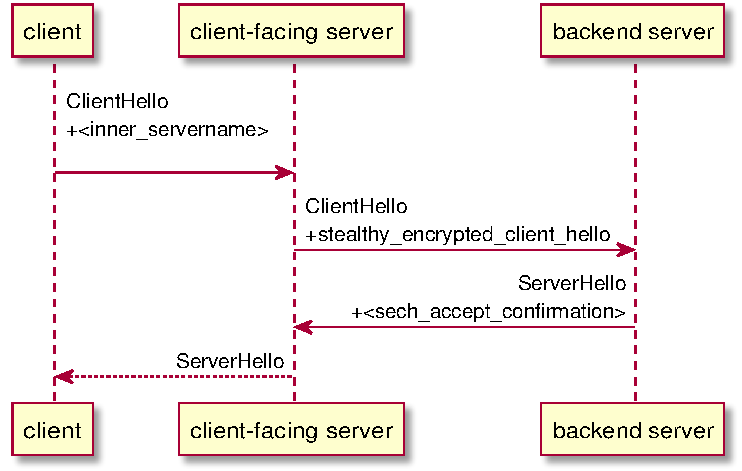
\includegraphics[width=\linewidth]{figure/sech-split-mode-accept.pdf}
\captionsetup{width=.8\linewidth} 
\caption[]{Sequence diagram for a successful SECH split-mode handshake.}
\label{fig:sech-split-mode-accept}
\end{figure}

\section{SECH 1: Secretless Stealthy Encoding}
\subsection{Motivations and Deployment Scenarios}

[ ] more properly should be called just `stealthy SNI' or `stealthy CH', because this version does not use encryption

[ ] very low coordination/infrastructure requirements to get this working

[ ] SECH.1 does **not** offer confidentiality of the SNI or ALPN, aim here is purely censorship circumvention, not privacy

[ ] as a censorship circumvention method this can be easily detected and prevented

[ ] possibly useful ephemerally and at a small scale

[ ] circumvention in depth: use lots of different circumvention methods (including this insecure one) in order to increase the cost of censorship
\subsection{Design}
\subsection{Implementation Notes}


\section{SECH 2: Static Secret Shared OOB}
\subsection{Motivations and Deployment Scenarios}

The amount of `cover' available in the TLS 1.3 \var{ClientHello} message in which we can hide information without differentiating the message from an a normal TLS 1.3 message is limited. By using only a symmetric encryption algorithm as the basis for sending the stealthy information there is a smaller overhead than there would be with PKC or HPKE.

With the \var{random} and \var{legacy\_session\_id} fields we get a contiguous sequence of 64 octets. Other fields/extensions with values that {\em may} look random (and thus might provide cover) are the cipher suite GREASE values, the PSK identity, the \var{key\_share} itself. However, the cover provided by these fields/extensions would be less certain because they differ across situations/implementations of TLS. Using these effectively as cover for stealthy bits would involve mimicking the behaviour of a specific implementation in order not to stick out.

[ ] if the client and server can share the OOB secret securely then we can implement a highly stealthy and cryptographically secure inner SNI

[ ] since the server does not have to publish a public key (as in ECH), it is possible to hide the fact that the server is support SECH from all except the client who knows the OOB secret

[ ] the secret could be shared amongst multiple clients, allowing for some scale of deployment, but this protocol is certainly not appropriate for internet scale deployments (millions of clients). The more widely the secret is shared the more likely it is to be leaked.

[ ] This design is NOT forward secret. If the shared secret is compromised then 

\subsection{Design}

We assume the client and client-facing server have some way to securely share a secret out-of-band; call this secret $s$ or \var{sech2\_long\_term\_key}. The shared secret should be a random string of at least 32 octets, or a longer string with at least that much entropy.


The client wishes to communicate \var{sech\_inner\_servername} secretly and stealthily to the client-facing server. Due to the limited amount of `cover' in the \var{ClientHello} the maximum length of \var{sech\_inner\_servername} is \sechtwoservernamelen. The \var{sech\_inner\_servername} is padded with a suffix of zeros to yield \var{padded\_servername} which is \sechtwoservernamelen octets long.  The client also generates a session-specific \sechtwoivlen{} octet \nonce. The plain text for encryption $pt$ is the \sechtwoservernamelen{} octet \var{padded\_servername}.
The session SECH 2 encryption key $sk_c$=\var{sech\_session\_secret} is computed as defined in \ref{lst:sech2-derive-secret}.
The client should ensure that it has never used the $(\nonce,sk_c)$ pair before, but ensuring that $(\nonce,sk_c)$ are never reused globally may not be feasible. Ideally the $(\nonce,sk_c)$ should never be used twice by any clients, but if there a multiple clients that do not coordinate this will be impossible to guarantee.


We note that the \var{random} and \var{legacy\_session\_id} are contiguous giving us a contiguous string of 64 octets in which we hide the SECH 2 offer, and we call this contiguous string $c$ for `cover'. The AEAD encrypted text has length \sechtwocipherlen{} and is placed in bytes \sechtwocipheroffset{}  to \sechtwocipherend{} of $c$, as depicted in Figure~\ref{fig:sech2-cover}, yielding \var{\ClientHelloOuter}.

We define \var{ClientHelloOuterContext} as a clone of \var{ClientHelloOuter}, except with bytes 12 to 64 of the cover $c$ set to 0s. The session key $sk_c$ can only be computed after \var{Client\-HelloOuterContext} is known.
The secure derivation of $sk_c$ depends on the entropy of the \var{key\_share} extension included in \var{ClientHelloOuterContext}.
[ ] TODO: what if key\_share is not included, e.g. for PSK-only handshake? Reject SECH?

The additional authenticated data $aad$ is empty.

%the transcript of \var{ClientHelloInner} message, which is \var{ClientHelloOuter} but with: 1. the encrypted AEAD output replaced with the plain text \var{sech\_inner\_servername} and \var{sech\_inner\_random}, as well as 2. the \var{extension\_data} field of the \var{server\_name} extension set to all 0s with the same length as the cover value for \var{server\_name} (The backend server does not learn the cover SNI used). The AEAD MAC $t$ is left in \var{ClientHelloInner}.

\begin{listing}[htb]
\centering
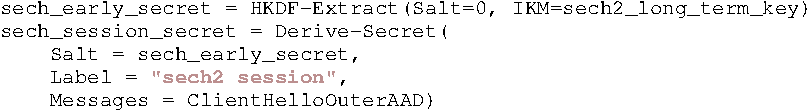
\includegraphics[width=\linewidth]{figure/sech2-derive-secret.pdf}
\captionsetup{width=.8\linewidth} 
\caption[SECH 2 Derive Secret]{Derive $sk_c$, the secret key that will be used by the client to encrypt $pt$ which has the inner \var{CH} data.}
\label{lst:sech2-derive-secret}
\end{listing}

The client encrypts $pt$ (authenticating $aad$) with $(\nonce,sk_c)$ using AES-128-GCM, producing a \sechtwotaglen{} octet authentication tag $t$ and the \sechtwocipherlen{} octet encrypted text $ct$. The \var{\ClientHelloOuter} has $c:=\nonce||ct||t$. The placement of the required values in cover $c$ of the \var{\ClientHelloOuter} is depicted in Figure~\ref{fig:sech2-cover}.

\begin{figure}[htb]
\centering
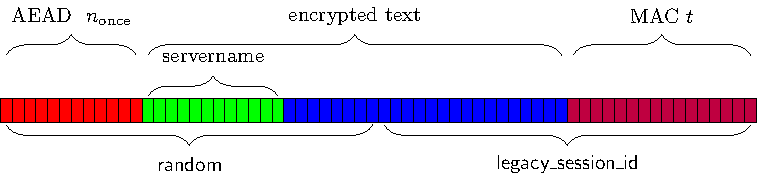
\includegraphics[width=\linewidth]{figure/sech2-cover.pdf}
\captionsetup{width=.8\linewidth} 
\caption[SECH 2 Cover]{Locations of AEAD inputs and outputs in the 64 contiguous octets of \var{ClientHello} \var{random} and \var{legacy\_session\_id}. The cipher text $ct$ and MAC tag $t$ outputs are a function of $iv$, $s$, $pt$, and $aad$: $(ct,t)=\text{AEAD}(iv,s,pt,aad)$.}
\label{fig:sech2-cover}
\end{figure}

A cooperating server in possession of $s$ that receives a \var{ClientHello} first constructs \var{ClientHelloOuterContext}, then $sk_c$, and should attempt to decrypt and authenticate $ct$. If decryption/authentication are unsuccessful the server continues with the TLS 1.3 handshake as normal. If successful, the client-facing server forwards \var{ClientHelloInner} to the backend server identified by the inner server name. If the inner server name does not identify a backend server then the client-facing server continues the TLS 1.3 handshake as if SECH 2 is disabled.

The \var{ClientHelloInner} message  is \var{ClientHelloOuter} but with: 1. the encrypted AEAD output $ct$ replaced with the plain text $pt$, as well as 2. the \var{extension\_data} field of the \var{server\_name} extension set to all 0s with the same length as the cover value for \var{server\_name} (The backend server does not learn the cover SNI used). The AEAD MAC $t$ is left in \var{ClientHelloInner}.

The backend server can distinguish a \var{ClientHelloInner} from a regular regular \var{ClientHello} by the \var{server\_name} extension. If the \var{extension\_data} field of the \var{server\_name} has all 0s it is a \var{ClientHelloInner}. Otherwise it should be treated as a regular TLS 1.3 hello.

The server parses the plaintext $pt$ to retrieve the inner server name in order to select an identity. At this point the backend server might respond with \var{HRR} or \var{ServerHello}. Whereas in ECH the acceptance signal is always sent in the server's first message (whether it is a \var{HRR} or \var{SH}), for SECH 2 the acceptance signal is always in the \var{SH}. The client-facing server forwards these (and subsequent) messages to the client unaltered. In the case of \var{HRR} the backend server creates a normal \var{HRR} response and the client constructs \var{ClientHello2} as specified in RFC 8446 (\cite{rfc8446}). If the backend server accepts the parameters of \var{ClientHello} (or \var{ClientHello2} in the case of \var{HRR}) and accepts the inner servername identified in $pt$, then it responds with a special \var{ServerHello} containing an SECH acceptance signal. Also, if using certificate-based authentication, then the later \var{Certificate} message should contain a certificate identified in $pt$.

The SECH 2 acceptance signal is 8 octets long and placed in the last 8 bytes of the \var{ServerHello.random}. It is a function of the transcript of the handshake so far, \var{sech\-\_\-transcript\_hash}, and $s=$\var{sech2\_long\_term\_key}. We define \var{sech\_accept\_confirmation} in Listing~\ref{lst:sech2-accept-function} and \var{sech\_transcript\_hash} in Listing~\ref{lst:sech2-transcript-hash}.

\begin{listing}[htb]
\centering
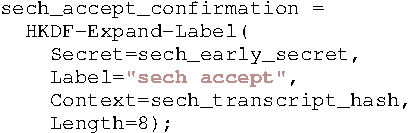
\includegraphics[width=.7\linewidth]{figure/sech2-accept-function.pdf}
\captionsetup{width=.8\linewidth} 
\caption[SECH 2 Accept Confirmation]{The function used to calculate the SECH 2 acceptance signal using the \var{HKDF-Expand-Label} function defined in Section 7.1 of RFC 8446 (\cite{rfc8446}). The \var{sech\_early\_secret} is derived from $s$ as defined in Listing~\ref{lst:sech2-derive-secret}, and \var{sech\_transcript\_hash} is described in Listing~\ref{lst:sech2-transcript-hash}.}
\label{lst:sech2-accept-function}
\end{listing}

\begin{listing}[htb]
\centering
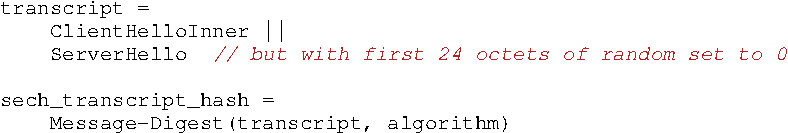
\includegraphics[width=\linewidth]{figure/sech2-transcript-hash.pdf}
\captionsetup{width=.8\linewidth} 
\caption[SECH 2 Transcript Hash]{Specification of the \var{sech\_transcript\_hash} used to calculate \var{sech\_accept\_confirmation}. The \var{algorithm} is the hash algorithm of the negotiated cipher suite for the handshake.}
\label{lst:sech2-transcript-hash}
\end{listing}

% The client uses that secret to encrypt the true target servername as well as a 32 byte secret inner nonce which are hidden in the ClientHello \var{random} and the \var{pre\_shared\_key} extension. The inclusion of the secret inner nonce is necessary to mitigate cut-and-paste attacks.

% More precisely, the client generates a 12 byte initialisation vector for AES-128-GCM. The plaintext is an ASCII encoding of the servername padded with 0x00 up to 12 bytes, appended to the 32 byte inner nonce.
% AEAD is used but the AAD is 0-length. % TODO: might be better to use the transcript hash of ClientHello (with random zeroed) as AAD, (however, if random is zeroed then transcript hash might not change)
% The AEAD tag is truncated to 8 bytes, such that we have a combined 64 bytes to send, which are put into the \var{ClientHello.random} and \var{ClientHello.legacy\_session\_id}. The first 12 bytes contain the IV, the next 12 contain the first 12 bytes of the cipher text, and the last 8 bytes of the \var{random} contain the truncated MAC, and the \var{ClientHello.legacy\_session\_id} is the last 

If the backend server accepts SECH 2 then it makes the SECH inner servername available to the application program via a callback or some other means, which allows the application program to decide whether or not to switch contexts (server certificate etc.).

\subsubsection{SECH 2 with PSK}
If a server accepts SECH 2 it may issue a ticket referencing a PSK that can be used to resume with backend server without stealthy encryption.

The PSK is derived as defined in Listing~\ref{lst:sech2-psk}, which differs from the definition of the PSK defined RFC 8446 in that the label is \var{``sech res''} rather than \var{``resumption''}. This ensures that the standard TLS 1.3 PSK is only used for a connection to the outer servername, whereas the \var{sech2\_psk} is only used for the inner servername.
\begin{listing}
\begin{verbatim}
sech2_psk = HKDF-Expand-Label(
    resumption_master_secret,
    "sech res",
    ticket_nonce,
    Hash.length)
\end{verbatim}
\caption{\label{lst:sech2-psk}Definition of the PSK used when resuming an SECH 2 session.}
\end{listing}

Note that this definition of \var{sech2\_psk} is a function of the \var{resumption\_master\_secret}, which is not available to a client-facing server in split-mode.
Therefore, this type of resumption is not possible in split-mode. % TODO: design PSK resumption for split mode
% TODO: what if sech2_psk and psk are the same, e.g. because they collide when using different ticket_nonces? maybe the label should still be "sech res" but each ticket_nonce should be marked as either sech or non-sech?

To use a resumption PSK (sent via \var{NewSessionTicket}) in TLS 1.3 the PSK has to be validated with a \var{BinderEntry} which binds the PSK cryptographically to the transcript of the first handshake as well as most of the \var{CH} for the second handshake. Pseudocode for this process is presented in Listing~\ref{lst:binder-pseudocode}, but this process is not used in SECH 2, as explained below.

\begin{listing}
    \begin{verbatim}
early_secret = HKDF-Extract(0, PSK)
binder_key = Derive-Secret(early_secret, "res binder", "")
binder_finished_key = HKDF-Expand-Label(
    binder_key,
    "finished",
    "",
    Hash.length)
binder =
    HMAC(binder_finished_key,
        Transcript-Hash(
            HandshakeContext1..ClientHello))
    \end{verbatim}
    \captionsetup{width=.8\linewidth} 
    \caption{\label{lst:binder-pseudocode}Pseudocode of the process used to compute a \var{binder} when using a resumption PSK. The \var{HandshakeContext1} is the transcript of the handshake in which the PSK was derived, and \var{ClientHello} is for a new connection and is truncated so as not to include the \var{binders} list itself. This formulation is tweaked slightly in the case of SECH 2.}
\end{listing}

\subsection{Distributing SECH 2 access without sharing \var{sech2\-\_long\-\_term\_secret}}
[ ] TODO research has anyone done ticket sharing amongst clients before? E.g. client with multiple processes

[ ] TODO bleichenbacher attack

Sharing the SECH 2 long term secret widely amongst clients would violate the `Avoid Widely Shared Secrets' requirement advocated by \citep{rfc8744-issues}. How do we facilitate connections from large numbers of clients while restricting each long term secret to being shared to only 2 parties? One option is to have a distinct long term secret for each client-server pair. The SECH 2 design specified here can facilitate this through trial decryption, i.e. every \var{ClientHello} processed by the server is checked against each registered secret until one is found to successfully decrypt the inner server name. This approach scales horribly, with the cost of every connection being proportional to the number of registered clients, whether or not those clients are active. But note that this trial decryption process is highly parallelizable.

Another approach is to modify the TLS 1.3 session resumption mechanism in order to allow a client to distribute PSKs to other clients. Those other clients could then resume the first client's session in order to access the backend server.

When a servers generates a \ac{PSK} and shares it in a \ac{NST} message, then (in TLS 1.3) \ac{PSK} is of type ``resumption'', rather than ``external''. Using ``resumption'' tickets/\acp{PSK} has a few extra steps compared to ``external'' \acp{PSK}. The calculation of the \var{binder} when using ``resumption'' incorporates the transcript of messages from the first session as well as initial messages from the new session, whereas without an external \ac{PSK} there is no `first' session so the transcript is just of the first session.

We consider now the scenario where a client (C1) completes an SECH 2 handshake in order to establish a PSK, but wishes to pass the PSK to a different client (C2) so that C2 can connect to the backend server stealthily without knowing the \var{sech2\_long\_term\_key}. One approach would be to treat the \ac{PSK} as ``resumption'' type. This would require the \var{binder} value in Listing~\ref{lst:binder-pseudocode} which is a function of the PSK and the transcript up to and including the new \var{ClientHello}. For resumption \acp{PSK} \var{Handshake Context 1} is the transcript of the first session's handshake, whereas for external \acp{PSK} \var{Handshake Context 1} is the empty string. Typically the \var{HandshakeContext1} is private because it contains decrypted confidential handshake messages, and therefore should not be shared with the other untrusted client C2. At the same time, in order to compute a valid \var{ClientHello} the private component of the \var{key\_share} is needed, and this value should not be accessible to C1 when C2 is resuming the session. In other words C1 should have exclusive access to the first part of the transcript, and C2 must generate the second part of the transcript. Therefore, in order to calculate the \var{binder} while maintaining these rules C2 would have to send the new \var{ClientHello} to C1. This is highly inconvenient operationally; it means that C1 would have to remain live and accessible in order for C2 to use the \ac{PSK}. For these reasons we deem that using \acp{PSK} of type ``resumption'' to bootstrap a second client is not viable.

\begin{listing}
    \begin{verbatim}
binder =
    HMAC(binder_key,
        Transcript-Hash(Handshake Context1,
        ClientHello) )
    \end{verbatim}
    \captionsetup{width=.8\linewidth} 
    \caption{\label{lst:binder-sech2-pseudocode}Normal calculation of \var{binder} in TLS 1.3.}
\end{listing}

While binding the bootstrap \ac{PSK} to the session in which it was generated is desirable, and it would be more congruent with the existing TLS 1.3 spec (\acp{PSK} delivered by \ac{NST} are bound in this way), we instead opt to treat bootstrap \acp{PSK} more like `external' keys. The calculation of the \var{binder} is simplified as in Listing~\ref{lst:binder-sech2-pseudocode-ext}. By acquiring from C1 just the \ac{PSK} value itself and the associated hash algorithm C2 has enough information to use the \ac{PSK}.

\begin{listing}
    \begin{verbatim}
binder =
    HMAC(binder_key,
        Transcript-Hash(ClientHello))
    \end{verbatim}
    \captionsetup{width=.8\linewidth} 
    \caption{\label{lst:binder-sech2-pseudocode-ext}Calculation of \var{binder} for SECH 2 bootstrap \acp{PSK}.}
\end{listing}

%[ ] The server uses the 32 byte shared secret key as well as the decrypted inner servername to create an 8 byte acceptance signal which is hidden in the ServerHello.random. The 8 byte acceptance signal is computed as \var{sech\_accept\_confirmation = AEAD-encrypt(IV, plaintext="", aad=sech\_inner\_servername, accept\_key).tag}, where IV is the first 12 bytes of the ServerHello.random (uniformly randomly generated), the plaintext is zero-length, the AAD is precisely the inner servername (which does not need to be transmitted because it is known by the client), and \var{accept\_key} is a session-specific key derived using HKDF from the session's master secret and the transcript of ClientHello..ServerHello, but with the last 16 bytes of ServerHello.random set to 0x00. The last 8 bytes of \var{ServerHello.random} are possibly used for an ECH acceptance signal, and the ECH acceptance signal is computed based on the transcript of ClientHello..ServerHello, except with the last 8 bytes of of ServerHello.random set to 0x00. Therefore, if the server is sending an SECH acceptance signal *and* an ECH acceptance signal, the SECH acceptance signal is computed first because the ECH acceptance signal is defined to incorporate the SECH acceptance signal bytes in its transcript hash. To construct the 8 sech\_accept\_confirmation bytes we make use of the HKDF-Expand-Label function defined in RFC 8446 Section 7.1.
    % ```c
    % md = TranscriptHash(ClientHello..ServerHello) // with last 16 bytes of ServerHello.random set to 0x00
    % padded\_sech\_IV = pad(sech\_IV, HashLen)
    % sech\_accept\_confirmation = HKDF-Expand-Label(
    %   HKDF-Extract(padded\_sech\_IV, sech\_symmetric\_key),
    %   "sech ac" || 0x00 || sech\_decrypted\_inner\_servername,
    %   md,
    %   8
    % )
    % ```

\subsection{Design Differences Between SECH 2 and ECH}
[ ] The acceptance signal is always sent in the \var{ServerHello}

[ ] This definition of \var{sech\_accept\_confirmation} is essentially a modification of the ECH \var{accept\_confirmation} defined in Section 7.2 of [TODO cite ECH draft], which we repeat here:
% ```
%   accept\_confirmation = HKDF-Expand-Label(
%     HKDF-Extract(0, ClientHelloInner.random),
%     "ech accept confirmation",
%     transcript\_ech\_conf,
%     8
%   )
% ```

The ECH \var{accept\_confirmation} uses \var{HKDF-Extract(0, ClientHelloInner.random)} as the `Secret' passed to \var{HKDF-Expand-Label}, and \var{HKDF-Extract(0,ClientHelloInner.random)} is confidential (only known to the client and server) because the \var{ClientHelloInner.random} was in the {\em encrypted} \var{ClientHelloInner}. Also, it is essential that \var{accept\_confirmation} can be generated by the backend server in ECH split mode, which is why the salt passed to \var{HKDF-Extract} is the 0 string. While it would be more secure to use a session-specific random value as the salt for \var{HKDF-Extract}, we cannot use the \var{ClientHelloOuter.random} because this value is not available to the backend server (the backend server only processes the ClientHelloInner). The HKDF specification assumes that the salt and IKM passed to HKDF-Extract are indepedent of each other (Section 3.4 RFC 5869), and in particular that the salt values are not `chosen or manipulated by an attacker'.
Since \var{ClientHelloOuter.random} is never processed by the backend server it will not be incorporated into the \var{Finished} message, which means it is not protected from tampering in split-mode. This means an attacker could manipulate \var{ClientHelloOuter.random} and so it should not be used as the salt for \var{HKDF-Extract}.

[ ] In order to facilitate a split mode of operation in a similar fashion to ECH it must be possible for the SECH backend server to produce  the \var{sech\_accept\_confirmation} signal. For the signal described above this entails that the backend server must possess the \var{sech\_symmetric\_key}, meaning \var{sech\_symmetric\_key} would be shared amongst three parties; client, client-facing server, backend server. This violates one of the design requirements listed in Section 3.2 by \cite{rfc8744-issues}; Avoid Widely Shared Secrets.
% \subsection{Security Considerations}

[ ] High probability for situations where an attacker can guess the plaintext, or where there are only a small number of possible plaintexts (SNIs). How does this affect capacity to brute force the secret key? -> Does this mean the SNIs must also remain secret?

\subsection{Implementation Notes}

[ ] Error handling
\subsection{Testing}

\section{SECH 3}
\subsection{Motivations and Deployment Scenarios}
\subsection{Design}
\subsection{Implementation Notes}
\section{SECH 4}
\subsection{Motivations and Deployment Scenarios}
\subsection{Design}
\subsection{Implementation Notes}

\section{SECH 5}
\subsection{Motivations and Deployment Scenarios}

[ ] arbitrary access for new clients without coordination from server

\subsection{Design}

[ ] server produces an \var{SECHConfig} and corresponding private key for the KEM

[ ] client has to attain \var{SECHConfig} in order to offer SECH 5 in a \var{ClientHello}, can attain over DoH or some other means

[ ] client encapsulates an ephemeral key $k$ using the KEM and public key specified in \var{SECHConfig} producing \var{enc}

[ ] client pads the servername to \var{SECHConfig.servername\_length} producing \var{\paddedServername}

[ ] client encrypts the \var{padded\_servername} with the AEAD specified in SECHConfig, and with key $k$ and a \nonce which is the first 12 octets of the hash of \var{SECH5ClientHelloAAD}, and with \var{SECH5ClientHelloAAD} as AAD, producing \var{sech5\_cipher} which is the concatenation of the encrypted text and the tag $t$

[ ] \var{SECH5ClientHelloAAD} is the \var{ClientHello} but with the portion in which the AEAD cipher (encrypted text and tag) will be placed set to zero, the size and location of this region depends on \var{SECHConfig}

[ ] \var{SECH5ClientHelloAAD} is the \var{ClientHelloOuter} but with the \var{random} and \var{legacy\_session\_id} set to all 0s

[ ] client encodes \var{enc} and \var{sech5\_cipher} in the \var{ClientHello} \var{random} and \var{legacy\_session\_id} fields producing \var{ClientHelloOuter} as depicted in Figure~\ref{fig:sech5-cover}

[ ] the client-facing server attempts to decapsulate \var{enc} with the private key associated with \var{SECHConfig} retrieving $k$, on failure continues with normal TLS 1.3

[ ] the client-facing server computes \var{SECH5ClientHelloAAD} and the \nonce, and then attempts to decrypt $ct$ and authenticate with $t$, on failure continues with normal TLS 1.3

[ ] on success the client-facing server constructs \var{SECH5ClientHelloInner} by replacing $ct$ with $pt$ and setting the \var{extension\_data} of the \var{server\_name} extension to all 0s

[ ] client-facing server forwars \var{SECH5ClientHelloInner} to the backend server

[ ] the backend server proceeds with SECH 5 iff the \var{server\_name} extension has all 0s, otherwise continues with normal TLS 1.3

[ ] the backend server might respond with \var{HRR} or \var{ServerHello}, the \var{HRR} is constructed as normal, but the \var{ServerHello} contains a special \var{sech5\_accept\_confirmation} value in the last 8 octets of the \var{random}


\begin{figure}[htb]
\centering
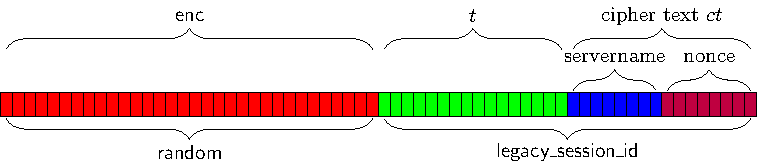
\includegraphics[width=\linewidth]{figure/sech5-cover.pdf}
\captionsetup{width=.8\linewidth} 
\caption[SECH 5 Cover]{}
\label{fig:sech5-cover}
\end{figure}

\subsection{Implementation Notes}

\section{SECH 6: TLS over TLS}
\subsection{Motivations and Deployment Scenarios}
\subsection{Design}
\subsection{Implementation Notes}


% At the beginning of each chapter, a description should introduce the reader to the content of the chapter. The description should explain to the reader the layout of the chapter, the contribution that the chapter makes to the overall dissertation and the contribution of the individual sections towards the overall chapter.


% \section{Problem Formulation}
% \label{sec:ProblemFormulation}

% This section should provide the reader with an overall description of the problem that will be addressed in the dissertation. In contrast to a generic discussion of the dissertation topic in the Introduction chapter, this section should provide a detailed discussion of the problem that has been identified based on the existing work that has been discussed in the preceeding chapter. 

% In some dissertations, it may make sense to convert this section into a short chapter of its own which follows the discussion of the existing work and preceeds the discussion of the work of the dissertation.

% \subsection{Identified Challenges}
% This section should present a short description of the gaps in the existing work and the relationship of these gaps to the work described in this dissertation.

% \subsection{Proposed Work}
% This section should provide a thorough description of the problem and an overview of the work proposed to address the problem.


% \section{Overview of the Design}
% \label{sec:OverviewOfDesign}
% A description of the approach that addresses the problem identified above.


% \section{Summary}
% \label{sec:SummaryDesign}

% Every chapter aside from the first and last chapter should conclude with a summary. 

\chapter{Implementation, Testing, and Deployment}

\section{Implementing an SECH API in OpenSSL}
\subsection{Introduction}
\subsection{Testing}
\subsection{Conclusions}
\section{Test Deployment}
\subsection{Introduction}
\subsection{Methods}
\subsection{Results}
\subsection{Discussion}

% \lstset{language=Python, captionpos=b, frame=single}
% \captionsetup{width=.8\linewidth} 


% Guess what? At the beginning of each chapter, a description should introduce the reader to the content of the chapter. The description should explain to the reader the layout of the chapter, the contribution that the chapter makes to the overall dissertation and the contribution of the individual sections towards the overall chapter.


% \section{Overview of the Solution}

% %% Short caption for the table of listings - long caption for the explanation for the reader
% \includecode{Sample Code}{Lengthy caption explaining the code to the reader}{lst:snippet}{snippet.py}

% The code in listing~\ref{lst:snippet} is a demonstration how to include a file with code into the template.



% \section{Component One}

% %% Defaults for listings

% The code in listing~\ref{lst:snippet2} is a demonstration how to include code in the template.

% %% Short caption for the table of listings - long caption for the explanation for the reader
% \begin{lstlisting}[caption={[Sample Code 2]Second Lengthy caption}, label={lst:snippet2}]
% x = 1
% if x == 1:
%     # indented four spaces
%     print("x is 1.")
% \end{lstlisting}


% \section{Summary}

% Every chapter aside from the first and last chapter should conclude with a summary. 


\chapter{Evaluation}
\label{chap:Evaluation}

\section{General Security and Privacy Considerations for SECH}

\subsection{Protocol Confidentiality}
As mentioned in Section~\ref{bleichenbacher-attack} any good \ac{SECH} protocol should protect the confidentiality of the fact that \ac{SECH} is being attempted and the fact that \ac{SECH} is supported. There are aspects of the protocol design that will protect this information, for instance how the connection continues with regular \ac{TLS} 1.3 whenever \ac{SECH} is aborted.
However, ensuring the confidentiality of this information depends also on
a careful and secure information. For instance, it may be possible for an attacker to somehow with high likelihood guess the library/implementation used for a particular channel. With this information the attacker could then analyse the timing of messages, or the particular alert messages under various circumstances to gain information about whether \ac{SECH} is in use.
The recurring discovery of \ref{bleichenbacher-attack}-style attacks are an attestation to the difficulty of implementing protocols that do not reveal such secret information.

To make matters worse, unlike \ac{RSA} private messages/keys which consist of many bits, the fact of a protocol being used/supported can be represented by a single bit, so protocol confidentiality is broken if an attacker can attain this single bit, meaning a successful attack will likely require much fewer oracle accesses than is the case for \ref{bleichenbacher-attack}. It should not be taken for granted that any given implementation of \ac{SECH} sufficiently protects protocol confidentiality.

% The Evaluation chapter should present a comparison of the work that forms the basis of the dissertation and existing work. At a higher level, it should demonstrate an awareness of the relationship of the dissertation work to the research area that it is based in.

% \section{Experiments}

% In the case where experiments have been carried out, the experimental setup and the values that were defined for the variables need to be presented in a table e.g. table~\ref{tab:experimentsetup}.

% \begin{table}[!h]
% \begin{center}
% 	\begin{tabular}{|l|c|c|} 
% 	\hline
%  	\bf Column 1  & \bf Column 2  & \bf Column 3 \\
%   	\hline
% 	Row 1 & Item 1 & Item 2 \\
% 	Row 2 & Item 1 & Item 2 \\
% 	Row 3 & Item 1 & Item 2 \\
% 	Row 4 & Item 1 & Item 2 \\
% 	\hline
% 	\end{tabular}
% \end{center}
% \caption[Variables of the experiment]{Caption that explains the table to the reader}	
% \label{tab:experimentsetup}
% \end{table}


% \section{Results}

% Figures that present results such as figure~\ref{fig:measurements} need to display descriptions of the axes, the units and scales of the measurements, statistical values, etc. Where measurements were taken from experiments, error bars or confidence intervals need to be provided to give the reader an indication of the spread of the measurements.

% \includescalefigure{fig:measurements}{Measurement of System Wakeups}{Long caption that describes the figure to the reader}{1}{measurements.png}


% \section{Summary}

% Every chapter aside from the first and last chapter should conclude with a summary that presents the outcome of the chapter in a short, accessible form. 
\chapter{Conclusions \& Future Work}
\label{chap:Conclusions}


\section{Future Work}

% This chapter should summarize the work presented in the dissertation and discuss the conclusions that can be drawn from the work and the results presented in chapter~\ref{chap:Evaluation}.


% \section{Future Work}

% The section may present a list of items that were beyond the scope of the dissertation.
\nocite{*}
% \begin{thebibliography}{refs}                   %% Start your bibliography here; you can
\addcontentsline {toc}{chapter}{Bibliography}     %% Force Bibliography to appear in contents
\bibliographystyle{apalike}
\bibliography{refs}                               %% also use the \bibliography command
%\end{thebibliography}                            %% to generate your bibliography.


%\addcontentsline {toc}{chapter}{Appendices}       %% Force Appendices to appear in contents
%\begin{appendix}
%\include{appendix1}
% \include{appendix2}
%\end{appendix}




\end{document}                                    %% END THE DOCUMENT
